\documentclass[a4paper,12pt, oneside]{book}

%\usepackage{fullpage}
\usepackage[italian]{babel}
\usepackage[utf8]{inputenc}
\usepackage{amssymb}
\usepackage{amsthm}
\usepackage{graphics}
\usepackage{amsfonts}
\usepackage{listings}
\usepackage{amsmath}
\usepackage{amstext}
\usepackage{engrec}
\usepackage{rotating}
\usepackage[safe,extra]{tipa}
\usepackage{showkeys}
\usepackage{multirow}
\usepackage{hyperref}
\usepackage{microtype}
\usepackage{enumerate}
\usepackage{braket}
\usepackage{marginnote}
\usepackage{pgfplots}
\usepackage{cancel}
\usepackage{polynom}
\usepackage{booktabs}
\usepackage{enumitem}
\usepackage{framed}
\usepackage{pdfpages}
\usepackage{pgfplots}
\usepackage[cache=false]{minted}
\usepackage{fancyhdr}
\pagestyle{fancy}
\fancyhead[LE,RO]{\slshape \rightmark}
\fancyhead[LO,RE]{\slshape \leftmark}
\fancyfoot[C]{\thepage}



\title{Sistemi distribuiti}
\author{UniShare\\\\Davide Cozzi\\\href{https://t.me/dlcgold}{@dlcgold}\\\\Gabriele De Rosa\\\href{https://t.me/derogab}{@derogab} \\\\Federica Di Lauro\\\href{https://t.me/f_dila}{@f\textunderscore dila}}
\date{}

\pgfplotsset{compat=1.13}
\begin{document}
\maketitle

\definecolor{shadecolor}{gray}{0.80}

\newtheorem{teorema}{Teorema}
\newtheorem{definizione}{Definizione}
\newtheorem{esempio}{Esempio}
\newtheorem{corollario}{Corollario}
\newtheorem{lemma}{Lemma}
\newtheorem{osservazione}{Osservazione}
\newtheorem{nota}{Nota}
\newtheorem{esercizio}{Esercizio}
\tableofcontents
\renewcommand{\chaptermark}[1]{%
	\markboth{\chaptername
		\ \thechapter.\ #1}{}}
\renewcommand{\sectionmark}[1]{\markright{\thesection.\ #1}}
\chapter{Introduzione}
\textbf{Questi appunti sono presi a le lezioni. Per quanto sia stata fatta una revisione è altamente probabile (praticamente certo) che possano contenere errori, sia di stampa che di vero e proprio contenuto. Per eventuali proposte di correzione effettuare una pull request. Link: } \url{https://github.com/dlcgold/Appunti}.\\
\textbf{Grazie mille e buono studio!}
\chapter{Introduzione ai Sistemi Distribuiti}
In questo corso analizziamo i sistemi distribuiti, alla base di tutte le applicazioni software 
client/server, in cui è presente una comunicazione tra diversi host.

\begin{definizione}
Un sistema distribuito è un sistema nel quale componenti hardware e software, collocati in computer
connessi alla rete, comunicano e coordinano le loro azione  col passaggio di messaggi.\newline
Ogni processo ha quindi una parte di logica applicativa e una di coordinamento. 
\end{definizione}

\begin{definizione}
un sistema distribuito è un insieme di elementi autonomi di computazione che si 
interfacciano agli utenti come un singolo sistema "coerente".
\end{definizione}

\begin{figure}
    \caption{Rappresentazione dei sistemi distribuiti}
	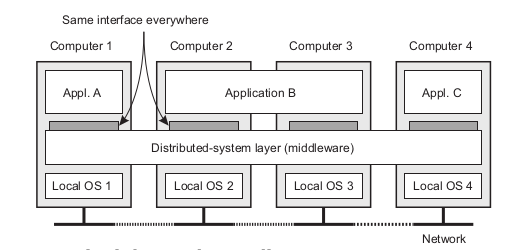
\includegraphics[scale=2.5]{img/cli.png}
\end{figure}
Le unità di computazioni sono dei nodi, i quali possono essere device hardware e/o singoli processi software,
autonomi che devono essere sincronizzati e coordinati(programmazione concorrente).\newline
Gli utenti e le applicazioni vedono un singolo sistema, senza conoscere le varie segmentazioni 
e i nodi presenti, e ciò permette di effettuare la \textbf{trasparenza di distribuzione}, 
ossia si nascondono i dettegli agli utenti che possono ignorare e non possono modificare il servizio.\newline 
In teoria con ciò si dovrebbe evitare la generazione degli errori, in quanto i nodi sono
indipendenti, ma in pratica tutto ciò è difficile da fare.

In un sistema distribuito, in quanto la comunicazione avviene tramite messaggi, non è presente la memoria
condivisa e non si ha un clock globale del sistema, ma ogni nodo si gestisce attraverso un clock interno.

\begin{center}
	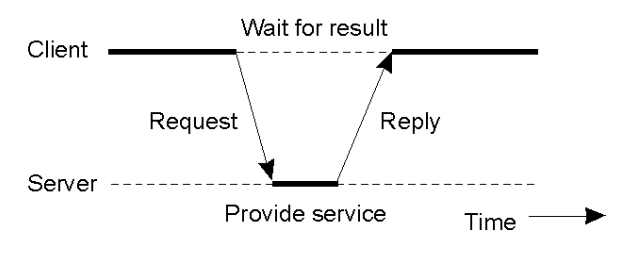
\includegraphics[scale=0.6]{img/cli2.png}
\end{center}
Si ha che un client fa una richiesta e il server risponde con un certo risultato (con il conseguente ritardo, a differenza del modello a chiamata di procedura).
\begin{center}
	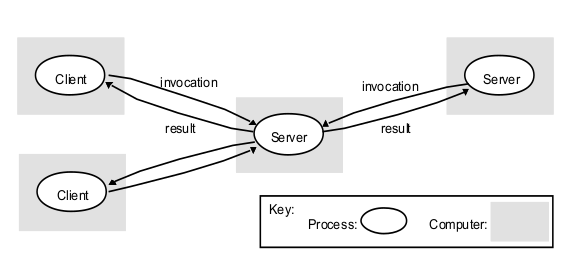
\includegraphics[scale=2.6]{img/cli3.png}
\end{center}
Si può accedere a server multipli (cluster con anche bilanciamento del carico) e si può accedere via proxy (dei server "finti" che fungono da concentratori).\\
Un sistema distribuito per comunicare effettua le seguenti operazioni:
\begin{enumerate}
    \item \textbf{identifica la controparte}, attraverso l'assegnazione di un nome(\emph{naming})
    \item \textbf{si accede alla controparte}, attraverso un punto di accesso
    \item \textbf{si definisce il protocollo}, al fine di stabilire le regole e le procedure per 
        essere in grado di comunicare, senza alcun problema.
    \item \textbf{si definisce}, che si risolve concordando \textit{sintassi e semantica} per l'informazione da condividere \textbf{(quest'ultimo è però ancora un problema aperto)}
\end{enumerate}

Si hanno le seguenti definizioni per quanto riguarda la trasparenza:
\begin{itemize}
    \item naming, si usano nomi simbolici per identificare le risorse,
            facenti parte del sistema distribuito.
    \item access trasparency, nascondere le differenze nella rappresentazione 
        delle informazioni e nell'accesso ad un'informazione locale o remota 
    \item location trasparency, in cui si nasconde dove è collocata una risorsa sulla rete
    \item  relocation(mobility) transparency, in cui si nasconde se la risorsa è stata
        trasferita ad un'altra locazione, mentre è in uso.
    \item migration trasparency, in cui si nasconde che una risorsa può essere trasferita
    \item replication transparency, in cui si nasconde che una risorsa può essere replicata
    \item concurrency transparency, in cui si nasconde che una risorsa può essere condivisa
        da molti utenti indipendenti
    \item failure trasparency, in cui si nascondono fallimenti e recovery di una risorsa
    \item persistence trasparency, in cui si nasconde se una risorsa
                  è volatile o memorizzata permanentemente
\end{itemize}
Da questa trasparenze non si è in grado di nascondere i ritardi e le latenze di comunicazione, ma
soprattutto non si è in grado di effettuare una trasparenza completa, per motivi di performance
e di latenza dell'operazioni su un sistema distribuito.

Questa volonta di astrarre le informazioni è alla base dell'ingegneria del software, in cui si separa
il \textit{cosa} dal \textit{come}: il cosa si effettua tramite la definizione dell'interfaccia, complete
ed indipendenti dalle diverse implementazioni, mentre il come avviene con l'effettiva implementazione
delle classi e dei metodi.\newline
Come si vede nella figura \href{figura:interfaccia}, l'interfaccia è unica mentre l'implementazione
varia in ogni host locale del sistema distribuito e ciò può essere anche visto come la separazione
tra un meccanismo e una politica, ossia come si implementa effettivamente una funzionalità del sistema.

\begin{figure}
    \caption{Interfaccia di un sistema distribuito}
    \label{figura:interfaccia}
    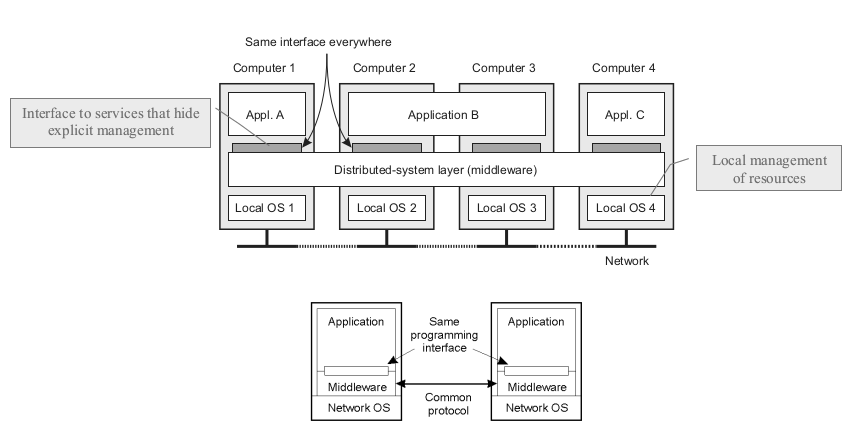
\includegraphics[scale=2]{img/cli4.png}
\end{figure}

\begin{figure}
    \caption{Immagine a caso}
	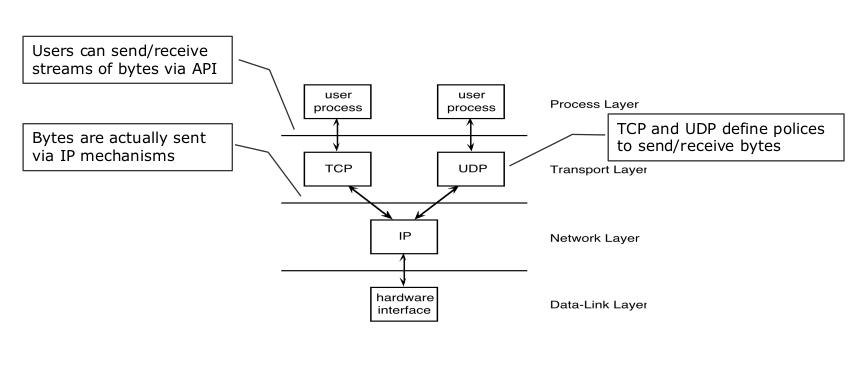
\includegraphics[scale=2]{img/cli5.png}
\end{figure}
Per poter capire le richieste ed eseguire i processi di comunicazione i due processi devono concordare 
un protocollo, in cui viene definito il formato, l'ordine di invio e di ricezione dei messaggi tra 
i diversi disposizioni, e per vedere un esempio di una comunicazione tra i diversi processi si guardi
il listato di codice \href{listato:fileServer}, in cui si implementano sia l'header che l'implementazione
del server mentre nel listato di codice \href{listato:fileClient} si vede l'implementazione del client.

Non forniamo una spiegazione del codice dato che nel corso del corso impareremo come sviluppare ed
implementare applicazioni client-server.

\begin{figure}
    \label{listato:fileServer}
    \inputminted{c}{code/header.h}
    \inputminted{c}{code/fileServer.c}
\end{figure}

\begin{figure}
    \label{listato:fileClient}
    \inputminted{c}{code/fileClient.c}
\end{figure}

\subsection{Stream Communication}
\begin{figure}
    \label{figure:livelliRete}
    \centering
    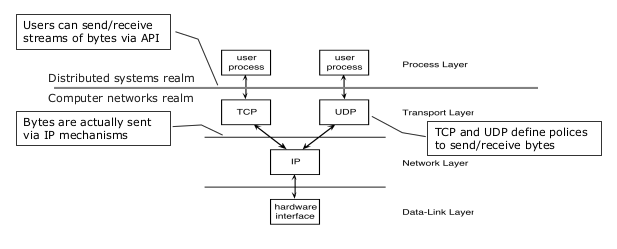
\includegraphics[scale=2.5]{img/sc.png}
\end{figure}
Per la comunicazione tra due host si utilizza il modello ISO/OSI, basato sull'astrazione di cui tutti gli
informatici ne dovrebbero conoscere in dettaglio tutti i vari livelli, in cui per mandare dei dati da un host
ad un host si parte dal livello di applicazione, su cui si sviluppano ed operano i sistemi distribuiti,
per poi andare ai livello di trasporto, di rete e fisico, necessari per il trasferimento sulla rete 
delle informazioni, come si nota nella figura \href{figure:livelliRete}.

Ogni processo comunica attraverso canali, in cui vengono gestiti i flussi di dati in ingresso ed uscita,
individuabili tramite un intero detto \textbf{porta} e noi studiamo le \textbf{socket}, particolare canale
per la comunicazione in cui non vi è una condivisione della memoria e per potersi connettere da un processo A,
il processo B deve conoscere l'host che esegue A e la porta in cui A è connesso.

Le socket possono essere principalmente di due tipi, come i principali protocolli di trasporti:
\begin{itemize}
    \item \textbf{tcp socket}: utilizzano il protocollo TCP, orientato alla connessione,
        per la comunicazione tra i due processi, prevede un controllo di affidabilità dei messaggi,
        ossia viene assicurato che i messaggi arrivano nell'ordine previsto all'altro processo
        ed infine vi è un controllo di flusso e di congestione ma non si hanno garanzie di banda e dei ritardi.

        Si utilizzano nelle applicazioni, in cui si deve avere la sicurezza dell'arrivo dei dati come ad
        esempio nel protocollo HTTP, per la comunicazione web, e nelle chat app come Telegram e Whatsapp.

    \item \textbf{udp socket}: utilizza il protocollo UDP, non affidabile e non orientato alla connessione,
        in cui viene solo garantito il trasferimento dei dati dalla rete all'applicazione e un controllo 
        minimale degli errori, cosa che lo definisce come un sottoinsieme proprio del protocollo TCP.\newline
        Viene utilizzato quando si deve avere un ritardo di trasmissione limitato ed una perdità minimale
        può non essere un problema, come ad esempio nei file multimediali e/o chiamate via voip.
\end{itemize}
Nei sistemi distribuiti non è necessario conoscere il funzionamento dei protocolli di trasporto ma basta
considerare i servizi offerti e il fatto che si trasferiscono stream di byte, infatti
le socket sono delle API(Application Programming Interface) per accedere a TCP o UDP, in quanto due processi
nel modello client-server comunicano mediante esso.

Si hanno delle criticità riguardanti alle socket e al modello client-server:
\begin{itemize}
    \item gestione del ciclo di vita di cliente e server, attivazione/terminazione del cliente e del server
    \item identificazione e accesso al server
    \item comunicazione tra client e server
    \item ripartizione dei compiti tra client e server, che dipende dal tipo di applicazioni 
          e la scelta influenza le prestazioni in relazione al carico
\end{itemize}
Quando viene definito l'indirizzo del server, esso può essere una costante, inserito dall'utente oppure
inserendo un nameserver su cui si ricava l'indirizzo tramite il DNS(Domain Name Service) e questo comporta 
un basso livello di trasparenza dato che gli utenti devono conoscre l'indirizzo della rete e soprattutto 
parsare lo stream di byte nel message voluto.

La comunicazione TCP/IP avviene attraverso flussi di byte, dopo una connessione esplicita, attraverso
normali system call read/write:queste due syscall sono sospensive, ossia mettono il sistema in attesa,
e utilizzano un buffer per garantire la massima flessibilità, ad esempio la read definisce un buffer
per leggere N caratteri ma potrebbe ritornare dopo aver letto solo $k < n$ caratteri.

\begin{figure}
    \centering
    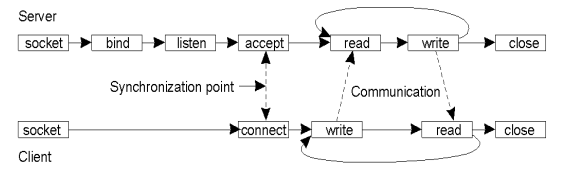
\includegraphics[scale=0.7]{img/sc2.png}
\end{figure}
Ci sono molte chiamate diverse per accedere i servizi TCP e UDP:
\begin{center}
	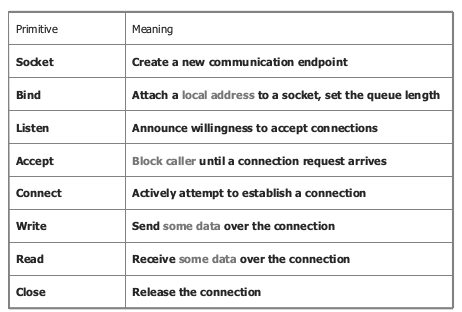
\includegraphics[scale=3]{img/sc3.png}
\end{center}
Per capire le operazioni e le procedure usate per permettere la comunicazione tra client e server,
mostriamo l'implementazione client-server con udp, nel listato \ref{udpSocket}, e quella
client-server tramite tcp, nel listato \ref{tcpSocket}.

\begin{figure}
    \caption{Implementazione socket con protocollo udp}\label{udpSocket}
    \inputminted{python}{code/udpClient.py}
    \inputminted{python}{code/udpServer.py}
\end{figure}

\begin{figure}
    \caption{Implementazione socket con protocollo tcp}\label{tcpSocket}
    \inputminted{python}{code/tcpClient.py}
    \inputminted{python}{code/tcpServer.py}
\end{figure}
Nelle socket udp, protocollo in cui si implementa un sottoinsieme delle funzionalità delle tcp, 
si effettua la creazione della socket, sia nel client che nel server, e poi subito incomincia la 
comunicazione mentre nelle socket tcp si effettua prima un handshake a tre vie per settare la connessione
tra client e server e poi incomincia la comunicazione.

\begin{figure}
    \caption{DIF A XASO}
	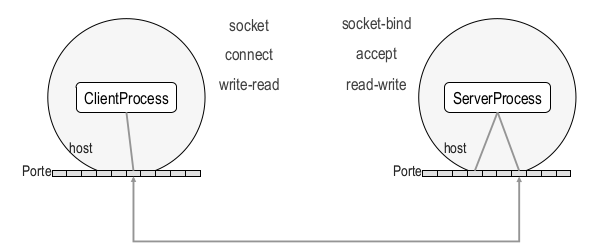
\includegraphics[scale=3]{img/sc4.png}
\end{figure}

\begin{minted}{c}
byteLetti read(socket, buffer, dimBuffer);
\end{minted}
con:
\begin{itemize}
	\item byteLetti = byte effettivamente letti
	\item socket = canale da cui leggere
	\item buffer = sapzio di memoria dove trasferire i byte letti
	\item dimBuffer = dimensione del buffer = numero max di caratteri che si possono leggere
\end{itemize}

Dopo aver mostrato come si implementano le socket in Python, per rendere semplice e facilmente comprensibile
quali sono le funzionalità e come si definiscono le socket, analizziamo come vengono fatte con il linguaggio
Java, usato nel corso, utilizzandoalcune classi che costituiscono un'interfaccia ad oggetti 
delle system call, su cui sono definite tutte le operazioni delle socket:
\begin{minted}{java}
    java.net.Socket
    java.net.ServerSocket
\end{minted}
Queste classi accorpano funzionalità e mascherano alcuni dettagli con il vantaggio di semplificarne l'uso
e come ogni framework è necessario conoscerne il modello e il funzionamento per poterlo usare efficacemente. 

I costrutti principali di queste due classi si possono trovare facilmente nella documentazione Java 
e negli esempi fatti a lezione, trovabili facilmente sul corso elearning.

Vediamo ora un esempio di un server \ref{java:tcpServer}, scritto in Java che accetta una connessione da un client 
e manda uno stream di dati, e di un client \ref{java:tcpClient}che legge lo stream di bytes, 
con un esempio similare a quello fatto in python per spiegare le fasi del TCP socket.

\begin{figure}
    \caption{Semplice implementazione TCP server in Java}
    \label{java:tcpServer}
    \inputminted{java}{code/javaSocket/ServerWriter/SenderServerSocket.java}
\end{figure}

\begin{figure}
    \caption{Semplice implementazione TCP client in Java}
    \label{java:tcpClient}
    \inputminted{java}{code/javaSocket/ServerWriter/ReceiverClientSocket.java}
\end{figure}

Quindi per il server si avrà la situazione \ref{img:javaServer} mentre nel client 
si verifica \ref{img:javaClient}.

Si nota facilmente che il seguente modello di client non funziona nella maniera corretta, per cui
si introducono i \textbf{lazy server} che mandano pochi byte per volta con un piccolo ritardo,
come si nota nel listato \ref{java:lazyServer}

\begin{center}
	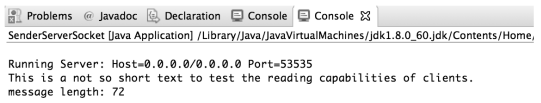
\includegraphics[scale=2.5]{img/sc5.png}
\end{center}
e per il client:
\begin{center}
	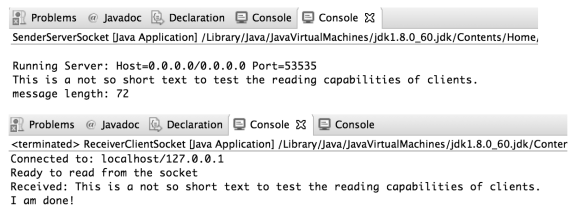
\includegraphics[scale=2.5]{img/sc6.png}
\end{center}

\begin{figure}
    \caption{Implementazione server Lazy}
    \label{java:lazyServer}
    \inputminted{java}{code/JavaSocket/ServerWriter/LazySenderServerSocket.java}
\end{figure}

\begin{center}
	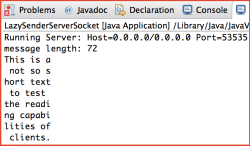
\includegraphics[scale=0.7]{img/lazy.png}
\end{center}
Per un'applicazione socket si ha le seguenti componenti:
\begin{enumerate}
	\item \textbf{client} con l'architettura che è concettualmente più semplice di quella di un server,
        spesso è un'applicazione convenzionale in cui si hanno solo effetti sull'utente client 
        e non comporta problemi di sicurezza.
	\item \textbf{server}: crea una socket, gli assegna una porta nota ed entra in ciclo infinito 
        in cui alternare: attesa di una richiesta, soddisfo la richiesta ed invio la risposta.\newline
	    L'affidabilità di un server è strettamente dipendente dall'affidabilità della comunicazione 
        tra lui e i suoi client, del resto però la modalità \textit{connection-oriented} determina 
        l'impossibilità di rilevare interruzioni sulle connessioni e la necessità di prevedere 
        una connessione (una socket) per ogni comunicazione.
\end{enumerate}
Ci sono diverse tipologie di server implementabili in un modello client-server:
\begin{itemize}
	\item iterativi, in cui viene soddisfatta una richiesta alla volta
	\item concorrenti processo singolo, in cui viene simulata la presenza di un server dedicato
	\item concorrenti multi-processo, in cui vengono creati server dedicati ad ogni client.
	\item concorrenti multi-thread, in cui vengono creati dei threat specifici per ogni client.
\end{itemize}
Vediamo come progettare un server iterativo. Al momento di una richiesta di connessione il server crea una
socket temporanea per stabilire una connessione diretta con il client: le eventuali ulteriori richieste
per il server verranno accodate alla porta nota per essere successivamente soddisfatte.\newline
Gli svantaggi sono che viene servito un cliente alla volta, il server impedisce l'evoluzione di molti
client e non si ha la scalabilità per cui la risoluzione a questi problemi è la programmazione concorrente.

Un server concorrente può gestire più connessioni client.
\begin{center}
	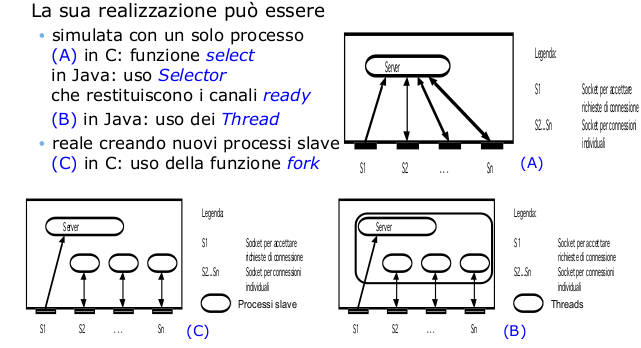
\includegraphics[scale=2.7]{img/conc.png}
\end{center}
In java si ha anche il \textbf{multiplexing} dove:
\begin{itemize}
	\item i \textbf{channel} possono operare sia in modalità bloccante che non bloccante. In modalità non bloccante (dove solo canali stream-oriented, come socket e pipe, possono essere usati) il channel non mette mai il thread invocato in sleep. L'operazione richiesta o viene completata completamente o ritorna che nulla è stato fatto
	\item si hanno classi speciali per java, come \textit{ServerSocketChannel, SocketChannel e
		      DatagramChannel} e si usano i selector, permettendo un controllo più fine dei socket channels.
\end{itemize}
Un Selector è un multiplexort di oggetti \textit{SelectableChannel} e viene creato con:
\begin{minted}{java}
Selector selector = Selector.open();
\end{minted}
I selector vengono poi registrati col metodo \textit{register}:
\begin{minted}{java}
channel.configureBlocking(false);
SelectionKey key = channel.register(selector, SelectionKey.OP_READ);
\end{minted}
Con le seguenti \textit{SelectionKey}:
\begin{minted}{java}
SelectionKey.OP_CONNECT // quando un client tenta di connettersi al server
SelectionKey.OP_ACCEPT // quando il server accetta la connessione del client
SelectionKey.OP_READ // quando il server è pronto a leggere dal canale
SelectionKey.OP_WRITE // quando il server è pronto a scrivere sul canale
\end{minted}
In generale ecco lo pseudo-codice per un server non bloccante:
\begin{verbatim}
create SocketChannel;
create Selector;
associate the SocketChannel with the Selector;
while(true) {
  waiting events from the Selector;
  event arrived;
  create keys;
  for each key created by Selector {
    check the type of request;
    isAcceptable:
      get the client SocketChannel;
      associate that SocketChannel with the Selector;
      record it for read/write operations
      continue;
    isReadable:
      get the client SocketChannel;
      read from the socket;
      continue;
    isWriteable:
      get the client SocketChannel;
      write on the socket;
      continue;
  }
}
\end{verbatim}
\newpage
ovvero:
\begin{center}
	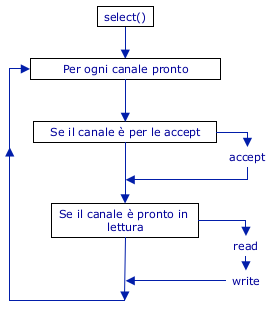
\includegraphics[scale=2.7]{img/conc2.png}
\end{center}
In java:
\begin{minted}{java}
import java.io.IOException;
import java.io.PrintWriter;
import java.net.InetAddress;
import java.net.Socket;
import java.util.Scanner;

public class SenderClient {
  private Socket socket;
  private Scanner scanner;

  private SenderClient(InetAddress serverAddress, 
    int serverPort) throws Exception {
    this.socket = new Socket(serverAddress, serverPort);
    this.scanner = new Scanner(System.in);
  }

  private void start() throws IOException, InterruptedException {
    String input;
    PrintWriter out = new PrintWriter(this.socket.getOutputStream(), true);
    while (true) {
      input = scanner.nextLine();
      if (input.contentEquals("exit"))
          break;
      out.print(input);
      out.flush();
    }
    System.out.println("Client terminate.");
    socket.close();
  }

  public static void main(String[] args) throws Exception {
    SenderClient client = new SenderClient(InetAddress.getByName(args[0]),
        Integer.parseInt(args[1]));

    System.out.println("Connected to: " + client.socket.getInetAddress());
    client.start();

  }

}

\end{minted}
\begin{center}
	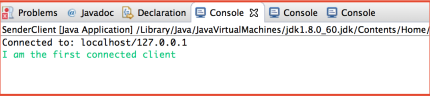
\includegraphics[scale=0.7]{img/conc4.png}
\end{center}
Vediamo come farlo in modo concorrente:
\begin{minted}{java}
package SelectorExample;

import java.io.IOException;
import java.net.InetSocketAddress;
import java.nio.ByteBuffer;
import java.nio.CharBuffer;
import java.nio.channels.SelectionKey;
import java.nio.channels.Selector;
import java.nio.channels.ServerSocketChannel;
import java.nio.channels.SocketChannel;
import java.nio.charset.Charset;
import java.nio.charset.CharsetDecoder;
import java.util.Iterator;
import java.util.Set;

public class ConcurrentServer {

  public static void main(String[] args) throws IOException {
    Selector selector = Selector.open();
    ServerSocketChannel server = ServerSocketChannel.open();
    server.bind(new InetSocketAddress("localhost", 53535));
    // set the channel in non blocking mode
    server.configureBlocking(false);
    // register the channel with the selector or the accept operation
    server.register(selector, SelectionKey.OP_ACCEPT);

    // Infinite server loop
    while (true) {
      // Waiting for events
      selector.select();
      // Get keys
      Set<SelectionKey> keys = selector.selectedKeys();
      Iterator<SelectionKey> i = keys.iterator();

      // For each keys...
      while (i.hasNext()) {
        SelectionKey key = (SelectionKey) i.next();

        // Remove the current key
        i.remove();

        if (key.isAcceptable()) // a client required a connection
          acceptClientRequest(selector, server);

        if (key.isReadable()) // ready to read
          readClientBytes(key);
      }
    }
  }

  private static void acceptClientRequest(Selector selector,
     ServerSocketChannel server) throws IOException {
    // get client socket channel
    SocketChannel client = server.accept();
    // Non Blocking I/O
    client.configureBlocking(false);
    // recording to the selector (reading)
    client.register(selector, SelectionKey.OP_READ);
    return;
  }

  private static void readClientBytes(SelectionKey key) throws IOException {
    SocketChannel client = (SocketChannel) key.channel();

    // Read byte coming from the client
    int BUFFER_SIZE = 256;
    ByteBuffer buffer = ByteBuffer.allocate(BUFFER_SIZE);
    try {
      if (client.read(buffer) == -1) {
        client.close();
        return;
      }
    } catch (Exception e) {
      // client is no longer active
      e.printStackTrace();
      client.close();
      return;
    }

    // Show bytes on the console
    buffer.flip(); // set the limit to the current position and then set 
      the position to zero 
    Charset charset = Charset.forName("UTF-8");
    CharsetDecoder decoder = charset.newDecoder();
    CharBuffer charBuffer = decoder.decode(buffer);
    int port = client.socket().getPort();
    System.out.println(port + ": " + charBuffer.toString());
    return;
  }
}

\end{minted}
\begin{center}
	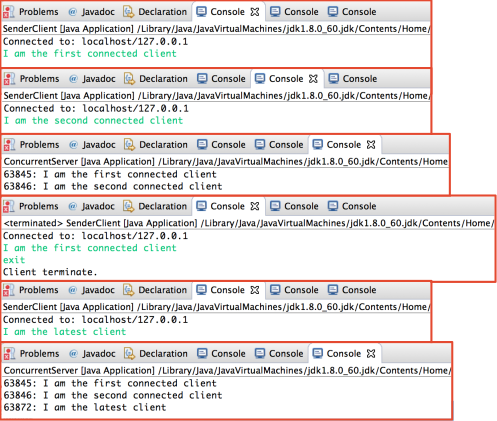
\includegraphics[scale=3]{img/conc5.png}
\end{center}
Vediamo anche una rappresentazione della chiamata di sistema fork:
\begin{center}
	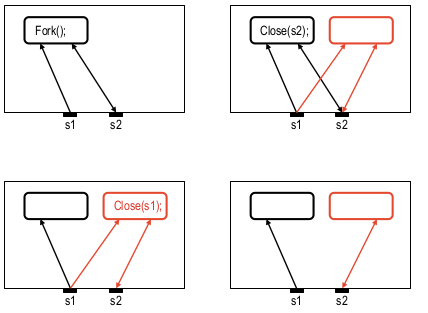
\includegraphics[scale=0.7]{img/fork.png}
\end{center}
La lettura/scrittura su una socket da parte di più processi
determina un problema di concorrenza: accesso ad una
risorsa condivisa (mutua esclusione). Si ha quindi;
\begin{center}
	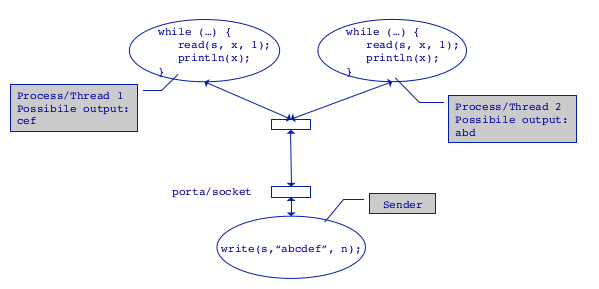
\includegraphics[scale=0.7]{img/ex.png}
\end{center}
Si hanno quindi 2 modelli:
\begin{enumerate}
	\item \textbf{mono processo (iterativo e concorrente)}, dove gli utenti condividono lo stesso spazio di lavoro. È adatto ad applicazioni cooperative che prevedono la modifica
	      dello stato (lettura e scrittura)
	\item \textbf{multi processo}, dove ogni utente ha uno spazio di lavoro autonomo. È adatto ad applicazioni autonome o che non modificano lo stato del server (sola lettura)
\end{enumerate}




















\subsection{Architettura dei server}
Per la gestione dei thread (che in java sono classi) esistono diversi \textbf{design pattern}:
\begin{itemize}
	\item \textbf{un thread per pattern}, dove il \textit{thread coordinatore} rileva la presenza di un nuovo client, lo connette ad un nuovo thread il quale:
	      \begin{itemize}
		      \item decodifica la richiesta
		      \item chiama la funzione servente che la soddisfa
		      \item torna in ciclo per leggere una nuova richiesta
	      \end{itemize}
	      \textbf{un thread per richiesta}, dove un \textit{thread coordinatore} riceve una richiesta e genera un thread per processarla. Questo nuovo thread:
	      \begin{itemize}
		      \item decodifica la richiesta
		      \item chiama la funzione servente che la soddisfa
		      \item termina
	      \end{itemize}
	\item \textbf{un thread per servente}, dove ogni servente ha un proprio thread e una coda. Il coordinatore riceve una richiesta e lo inserisce nella coda del servente giusto. Ogni thread servente legge ciclicamente una richiesta dalla
	      propria coda e la esegue
	\item \textbf{una pool di thread}, dove, dato che la creazione di un thread è costosa, il costo viene ammortizzato facendo gestire ad ogni thread molte richieste. Questo \textit{pool di thread} viene creato all'avvio del sistema e le richieste gli vengono assegnate man mano.
\end{itemize}

\section{L'architettura del web}
Per comunicare attraverso internet si utilizza un modello client-server usando principalmente 
il protocollo \textbf{HTTP}, attraverso l'esecuzione delle sue operazioni \textbf{request} e \textbf{response}:
la prima indica la richiesta di un oggetto web, come ad esempio un immagine e un file html, 
da parte del client verso il server mentre la seconda è la risposta da parte del server verso il client.

Nell'architettura di Internet il client viene realizzato mediante un browser, come ad esempio firefox,
programma che fornisce la possibilità di navigare sul web, attraverso l'interpretazione del codice
con cui sono espresse le pagine web, costituita da diversi oggetti identificati da un URL, mentre
il server viene fornito da un Web Server, come ad esempio Apache.

L'URL identifica un oggetto nella rete e specifica come interpretare i dati ricevuti 
attraverso il protocollo, è formato dai seguenti elementi:
\begin{itemize}
    \item nome del protocollo 
    \item indirizzo IP dell'host
    \item porta del processo
    \item cammino/percorso dell'host
    \item identificatore della risposta
\end{itemize}
rappresentata nel seguente modo
\begin{verbatim}
    protocollo://indirizzo_IP[:porta]/cammino/risorsa
\end{verbatim}
La parte testuale dei documenti viene espressa da HTML, per contenuti ed impaginazione, da CSS per 
il rending grafico mentre attraverso XML e JSON specifichiamo i dati e la loro struttura nel documento.

Si possono avere anche dati multimediali (foto, audio, etc...) con l'encoding MIME per definirne 
il formato (plain, html per i testi, jpeg, gif per le immagini, etc..) mentre la dinamicità delle pagine web
viene data da linguaggi di programmazione come Javascript, VBScript, Java/applet \dots .

Vi sono diversi protocolli web, in cui si definiscono le regole di comunicazioni tra varie tipologie di
applicazioni, come ad esempio HTTP, FTP(File Transfer Protocol) e SMTP(Simple Mail Transfer Protocol);
questi esempi di protocolli utilizzano il protocollo di trasporto TCP ed utilizzano delle porte note:
80 per HTTP, 20 per FTP e 25 per SMTP.

Per ora si hanno due versioni del protocollo HTTP, definite in maniera standard:
\begin{enumerate}
	\item\textbf{ http1.0: RFC 1945}
	\item\textbf{ http1.1: RFC 2068}
\end{enumerate}
HTTP è \textbf{stateless} in quanto il server non mantiene informazioni sulle precedenti richieste,
per cui si devono sempre fornire le informazioni necessarie per cui i siti web per avere informazioni 
utilizzano i cookie, che analizzeremo alla fine di questo paragrafo.\newline
Si ha che le \textit{request}e \textit{response} hanno la stessa struttura, in ASCII con un 
formato testo leggibile, ad esempio:
\begin{verbatim}
GET /somedir/page.html HTTP/1.1
Host: www.someschool.edu
Connection: close
User-agent: Mozilla/4.0
Accept: text/html, image/gif, image/jpeg
Accept-language: fr
\end{verbatim}
Con la prima riga si rappresenta la request line mentre nelle altre sono rappresentati l'header con le opzioni.

Nel protocollo HTTP si hanno diverse tipologie di metodi e richieste, le principali sono le seguenti:
\begin{itemize}
	\item \textbf{GET}: metodo HTTP, in cui viene restituita una rappresentazione di una risorsa web,
        senza effetti sul server, utile per ottenere pagine html ed immagini.

    \item \textbf{POST}: metodo HTTP, in cui vengono comunicati i dati da far elaborare al server oppure
        si crea una nuova risorsa, subordinata all'URL.\newline
        Ogni richiesta POST causa degli effetti sul server, quindi non può venire gestita la richiesta da 
        una cache e l'utilizzo tipico è quello per processare delle FORM html e di modificare 
        dati presenti in un database.
    
    \item \textbf{HEAD}: viene utilizzato spesso in fase di debugging ed è similare al metodo get
        ma in questo metodo viene restituito soltanto l'head della pagina web.
\end{itemize}
Nel complesso tutte le tipologie di richieste HTTP si notano nella figura \ref{fig:httpMethod} mentre 
il formato di una richiesta http si vede nella figura \ref{fig:httpStructure}.

\begin{figure}
    \caption{Tipologie di richieste HTTP}
    \label{fig:httpMethod}
	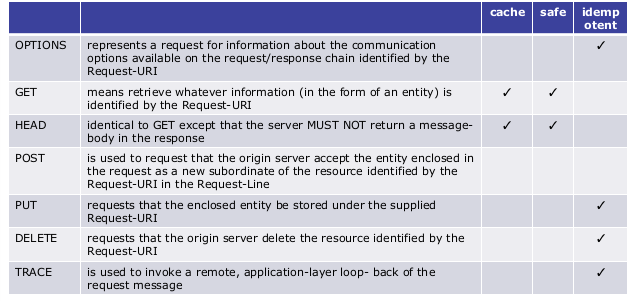
\includegraphics[scale=0.7]{img/http.png}
\end{figure}

\begin{figure}
    \caption{Formato di una richiesta HTTP}
    \label{fig:httpStructure}
	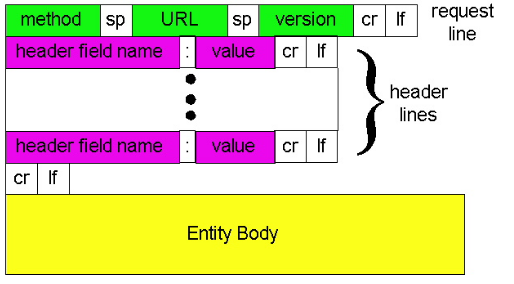
\includegraphics[scale=0.7]{img/http2.png}
\end{figure}
vediamo ora un esempio di risposta http:
\begin{verbatim}
HTTP/1.1 200 OK
Connection: close
Date: Thu, 06 Aug 1998 12:00:15 GMT
Server: Apache/1.3.0 (Unix)
Last-Modified: Mon, 22 Jun 1998
...
Content-Length: 6821
Content-Type: text/html
data data data data data ...
\end{verbatim}
In molte applicazioni web il client e il server comunicano per un periodo esteso, in cui il client
effettua una serie di richieste a cui il server risponde, in maniera intermittente oppure ogni tot 
periodo di tempo, per cui lo sviluppatore dell'applicazione deve decidere quale interazione deve
avvenire tra ogni richiesta, ossia se usare la stessa connessione TCP oppure crearne sempre una nuova;
la scelta comporta due diverse tipologie di utilizzo del protocollo HTTP, che si può estendere anche ai 
altri protocollo di livello applicativo:
\begin{itemize}
    \item \textbf{connessione non persistente}: quando il server manda l'oggetto richiesto viene 
        chiusa la connessione TCP, quindi successive interazioni tra lo stesso client e server richiedono
        la creazione e la chiusura di una nuova connessione TCP, con un aggravio di RTT, il tempo
        per mandare un pacchetto da client e server, per ogni richiesta solo per stabilire una nuova
        connessione TCP tra i due soggetti della comunicazione.

    \item \textbf{connessione persistente}: modalità usata di default dal protocollo HTTP, ma non per forza
        dagli altri protocolli, in cui al termine di una richiesta HTTP viene lasciata aperta la connessione
        TCP tra client e server, per cui ogni successiva richiesta tra essi non richiede la creazione
        di una nuova connessione, con conseguente maggiore efficenza e velocità del sistema.\newline
        Ovviamente la connessione TCP non viene lasciata aperta all'infinita, in quanto tipicamente 
        un server HTTP in caso di mancato utilizzo dopo un certo ammontare di tempo la chiude, per 
        raggiungere una maggiore efficienza di memoria occupata.
\end{itemize}
Esistendo due diverse versioni del protocollo HTTP vi sono due diverse tipologie di client:
\begin{itemize}
	\item Client HTTP 1.0: Server chiude connessione al termine della richiesta
	\item Client HTTP 1.1: mantiene aperta la connessione oppure chiude se la richiesta e quindi
	      contiene Connection: close, al fine di poter fare una connessione non persistente.
\end{itemize}
nella figura \ref{http:headerCode} alcuni esempi di codici, usati per stabilire il tipo di risposta 
effettuata da HTTP ed è importante saperli, per capire cosa è avvenuto quando riceviamo, come client,
la risposta HTTP.

\begin{figure}
    \caption{HTTP Header codes}
    \label{http:headerCode}
	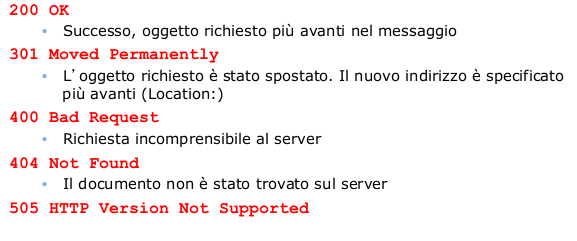
\includegraphics[scale=0.7]{img/http3.png}
\end{figure}
Nonostante il protocollo HTTP è di tipo stateless, per i siti web è comodo poter identificare una persona,
al fine di poter monitorare le abitudini, limitare l'accesso e personalizzare i contenuti, per cui sono 
stati introdotti i \textbf{cookies}, usati di default da tutti i siti.\newline
I cookie prevedono 4 componenti: una header line nel messaggio di risposta HTTP, un header line nel
messaggio di richiesta HTTP, un file di cookie tenuto nel sistema dell'utente e utilizzato dal browser,
infine un database back-end nel sito web.

Per capire come funzionano i cookie guarda la figura \ref{fig:cookie}, in cui si suppone che 
Susan accede al sito di Amazon per la prima volta, utilizzando nel header $Set-cookie: 1678$.\newline
Nonostante i cookie semplificano le procedure di riconoscimento dell'utente, come ad esempio 
si ha la possibilità di usare un applicazione e-mail senza doversi ogni volta registrare, 
ci sono alcuni aspetti negativi riguardo alla privacy, dato che tramite i cookies ed informazioni
ottenute sull'account di un utente, un sito web è in grado di sapere molto sull'utente e può 
vendere a terze parti, cosa che un utente vorrebbe sicuramente evitare.

La web cache, chiamata anche server proxy, è un rete in grado di soddisfare le richieste per conto di un
web server e possiede un suo storage sul disco, per tenere le copie degli oggett richiesti recentemente,
per cui si può configurare, come si nota nella figura \ref{fig:cache}, il browser affinche ogni richiesta 
HTTP venga dirottatta alla web cache, in cui in caso vi sia già una copia dell'oggetto viene subito 
mandata al browser, senza contattare il web server, altrimenti la web cache effettua una HTTP request
al web server e dopo aver ottenuto l'oggetto lo salva internamente e lo manda, tramite una HTTP response,
al browser che lo ha richiesto;come si può notare la web cache agisce sia da client che da server, infatti
quando interagisce con il browser è un server mentre quando comunica con il web server agisce come un client
e solitamente viene acquistata ed installata da un provider ISP.

La cache ha avuto un notevole utilizzo nel campo di internet per due ragione:
\begin{itemize}
    \item può ridurre il tempo di risposta di una richiesta client, in particolare se il collegamento
        tra client e web cache possiede una banda più potente del collegamento tra client e server
        e solitamente ciò avviene, e se si ha un alto tasso di possesso dell'oggetto richiesto da parte
        della cache, al fine di evitare continue richieste al web server.

    \item riduce il traffico sul link di accesso ad internet di una compagnia e/o istituzione, con la
        possibilità di evitare un upgrade della banda, con notevoli risparmi di costi.\newline
        Questa riduzione del traffico fornisce un guadagno anche agli utilizzatori delle applicazioni web
        dato che vi è un miglioramento delle prestazioni.
\end{itemize}
Nonostante la cache riduca il tempo di risposta, introduce il problema sulla integrità della copia
dell'oggetto rispetto a quella nel web server ma per risolvere il protocollo prevede un meccanismo, 
chiamato \textbf{conditional GET}, che permette alla cache di verificare se l'oggetto presente nel
suo storage interno è aggiornato.\newline
Un messaggio HTTP request prevede questo meccanismo in caso il messaggio usa il metodo GET ed 
include l'header \textbf{If-modified-since}, per cui la cache manda l'oggetto richiesto in caso 
in cui l'header if-modified-since coincide con il valore del header last-modified.

Per gestire l'accesso ai documenti sul server, dato che http è stateless, si deve verificare ogni richiesta 
e le informazioni necessarie all'autenticazione si trovano nell'header (\textit{authorization: line}) 
senza le quali il server rifiuta la connessione (\textit{www authenticate:}), come si nota 
nella figura \ref{img:authentication}.
\begin{figure}
    \caption{HTTP authentication}
    \label{img:authentication}
	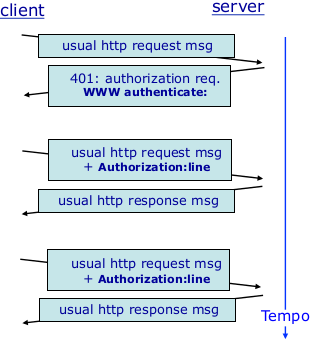
\includegraphics[scale=0.7]{img/http6.png}
\end{figure}
Quindi ricapitolando:
\begin{itemize}
	\item \textbf{applicazione}:
	\begin{itemize}
		\item invia i messaggi come stream di byte al servizio di trasporto
		\item legge lo stream di byte dal servizio di trasporto e ricostruisce i messaggi
\end{itemize}
	si ha quindi un unico messaggio:
	\begin{verbatim}
	GET /index.html HTTP/1.1<CR><LF>Host:
	   www.unimib.it<CR><LF>User-agent: Mozilla/4.0<CR><LF><CR><LF> 
	\end{verbatim}
	\item \textbf{servizio UDP}:
	\begin{itemize}
		\item scompone lo stream di byte ricevuto in segmenti 
		\item invia i segmenti, secondo una politica, ai servizi network
\end{itemize}
invia un messaggio così scomposto:
	\begin{verbatim}
	GET /index.html 
	HTTP/1.1<CR><LF>Host: ww
	w.unimib.it<CR><LF>U
	ser-agent: Mozilla/4
	.0<CR><LF><CR><LF>  
	\end{verbatim}
	\item \textbf{servizio TCP}: 
	scompone e invia come UDP e ogni segmento viene numerato per garantire
	\begin{itemize}
		\item riordinamento dei segmenti arrivati 
		\item controllo delle duplicazioni (scarto dei segmenti con ugual numero d'ordine)
		\item controllo delle perdite (rinvio dei segmenti mancanti) 
\end{itemize}
invia un messaggio così scomposto, con la numerazione del pacchetto all'inizio:
	\begin{verbatim}
	0GET /index.html 
	1HTTP/1.1<CR><LF>Host: ww
	2w.unimib.it<CR><LF>U
	3ser-agent: Mozilla/4
	4.0<CR><LF><CR><LF>  
	\end{verbatim}
	come in figura:
	\begin{center}
		
		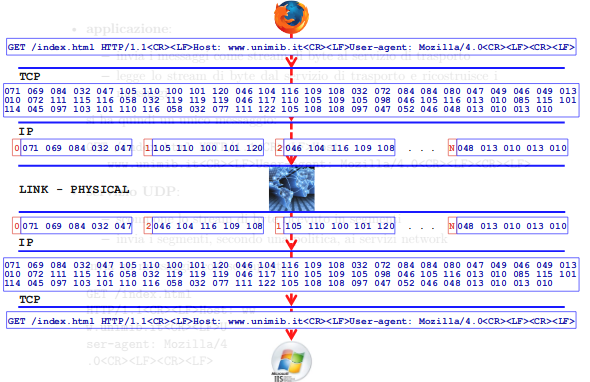
\includegraphics[scale=2.7]{img/send.png}
	\end{center}
\end{itemize}
\newpage
\subsection{Tipi di Comunicazione}
Si hanno 3 tipi di comunicazione:
\begin{itemize}
	\item \textbf{comunicazione asincrona}
	\item \textbf{comunicazione persistente}, dove il middleware memorizza i dati fino alla consegna del messaggio al destinatario e non è necessario che i processi siano in esecuzione prima e dopo l'invio/ricezione dei messaggi. Si divide in:
	\begin{itemize}
		\item sincrona:
		\begin{center}
			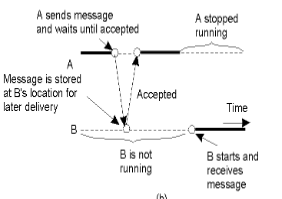
\includegraphics[scale=0.8]{img/sin.png}
        \end{center}
		\item asincrona:
		\begin{center}
			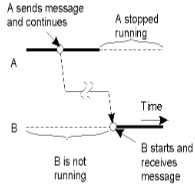
\includegraphics[scale=0.8]{img/asin.png}
		\end{center}
	\end{itemize}
	\item \textbf{comunicazione transiente}, ovvero se il destinatario non è connesso i dati vengono scartati. Si divide in:
	\begin{itemize}
		\item asincrona:
		\begin{center}
			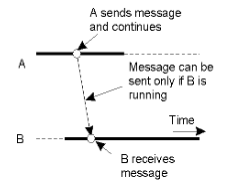
\includegraphics[scale=0.8]{img/asin2.png}
        \end{center}
		\item sincrona Receipt-based:
		\begin{center}
			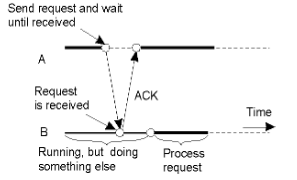
\includegraphics[scale=0.8]{img/sin2.png}
        \end{center}
        \item sincrona delivery-based:
        \begin{center}
			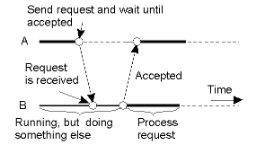
\includegraphics[scale=0.8]{img/sin3.png}
        \end{center}
        \item sincrona response-based:
        \begin{center}
			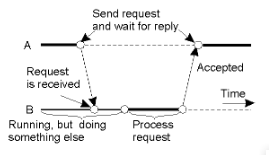
\includegraphics[scale=0.8]{img/sin4.png}
        \end{center}
	\end{itemize}
\end{itemize}
Vediamo un'immagine che spiega l'organizzazione generale di un sistema di comunicazione dove i vari hosts sono connessi attraverso la rete:
\begin{center}
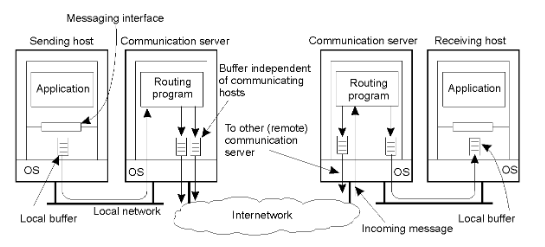
\includegraphics[scale=0.8]{img/host.png}
\end{center}
\subsubsection{Comunicazione Persistente message-oriented}
Si ha innanzitutto il \textbf{message-queeung model}. In questo caso si ha uno storage intermediario dei messaggi che non richiede ne il sender nel il receiver attivi durante la trasmissione:
\begin{center}
	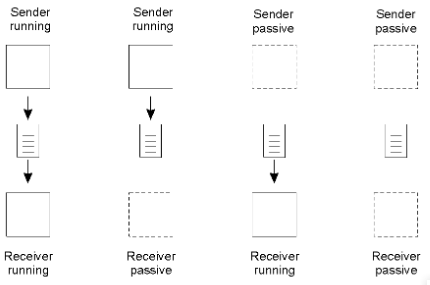
\includegraphics[scale=0.8]{img/que.png}
\end{center}
\begin{center}
	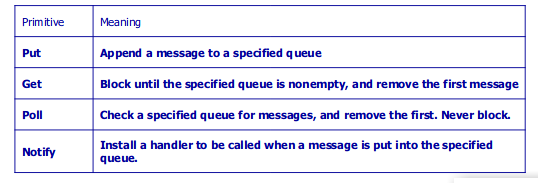
\includegraphics[scale=0.8]{img/queu2.png}
\end{center}
\begin{center}
	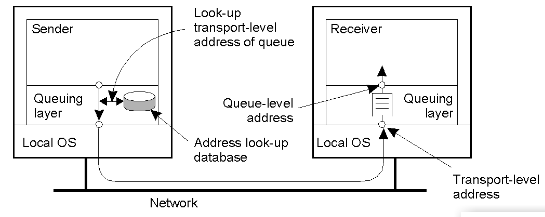
\includegraphics[scale=0.8]{img/queu3.png}
\end{center}
con i routers:
\begin{center}
	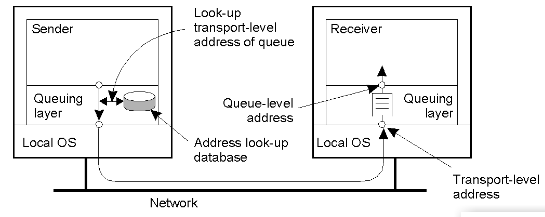
\includegraphics[scale=0.8]{img/queu3.png}
\end{center}
\section{Web Application}
Innanzitutto in un'applicazione web si ha l'adozione del protocollo HTTP. Si hanno dei limiti però nel protocollo HTTP a caratteri:
\begin{itemize}
	\item \textbf{lentezza}: occorre tradurre e ritradurre i dati 
	\item \textbf{uso di HTML per input e output}
	\item \textbf{uso di payload di tipo MIME}, quindi uso di interpreti esterni
\end{itemize}
Si hanno inoltre conversazioni senza stato (memoria), quindi ogni richiesta è un messaggio autonomo e per creare sessioni di lavoro (legare più richieste tra loro) occorre includere informazioni con mezzi espliciti , con \textit{cookie} o \textit{campi nascosti}.\\
Per realizzare una applicazione, il \textbf{Web Server} si fa aiutare da un \textbf{Application Server}. Un Application server è caratterizzato dal protocollo di interazione con il Web Server e l'interazione col client è sempre HTTP.\\
Lo sviluppo lato server si può avere sia con linguaggi compilati che con script interpretati. Nel caso di programmi compilati (un linguaggio qualsiasi che supporti l'integrazione col web server, C++, Java...) il web server si limita ad invocare, su richiesta del client, un eseguibile. Nel caso di esecuzione di script, il web server ha al suo interno un motore, \textit{engine}, in grado di interpretare il linguaggio di scripting usato (PHP, python, Perl...). In questo caso si perdono performances ma si guadagna una maggior semplicità di scrittura dei programmi.\\
Si hanno 3 step:
\begin{enumerate}
	\item URL definisce un naming globale
	\item GTTP fornisce un modello tipo RPC basato su socket e permette di invocare programmi sul server
	\item CGI (\textit{Common Gateway Interface}) permette al server di attivare un programma e di passargli le richieste e i parametri provenienti dal client 
\end{enumerate}
Ovvero:
\begin{center}
	\includegraphics[scale=0.7]{img/CGI.png}
\end{center}
Il processo CGI implementa un interprete per il linguaggio utilizzato coi vantaggi della portabilità, dell'utilizzo di strutture ben definite. Inoltre viene usato per programmare solo le logiche delle applicazioni. Tutto ciò si implementa con Java/Servlet, python e PHP. \\
\subsection{Il Lato Client}
Lato client si possono fare request \textbf{link-based} con il parametro \textit{action}:
\begin{minted}{html}
<body>
  <p>Click the link to ask the servlet to send back an HTML document</p>
    <a href="http://localhost:8080/SlideServlet/GetHTTPServlet"> 
      Get HTML Document      
    </a>
</body>
\end{minted}
Si ha quindi una richiesta del tipo: \textit{GET /path/name HTTP:1.1}\\
\begin{center}
	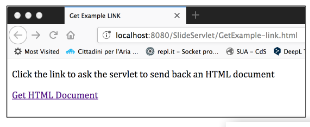
\includegraphics[scale=0.7]{img/lb.png}
\end{center}
Si possono fare richieste \textbf{form-based}:
\begin{minted}{html}
<form ACTION="http://localhost:8080/SlideServlet/GetHTTPServlet"
      METHOD="GET">
    <p>Click the button to have the servlet send an HTML document</p>
    <input TYPE="submit"VALUE="Get HTML Document">
</form>
\end{minted}
Si ha quindi una richiesta del tipo: \textit{GET /path/name HTTP:1.1}\\
\begin{center}
	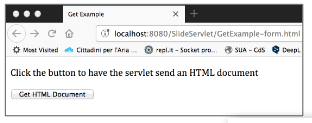
\includegraphics[scale=0.7]{img/fb.png}
\end{center}
Si ha anche che i dati possono essere inviati tramite un \textbf{FORM}:
\begin{minted}{html}
<form ACTION="http://localhost:8080/SlideServlet/PostHTTPServlet"
      METHOD="POST">  
  What is your favorite pet?<br><br>
  <input TYPE="radio"NAME="animal"VALUE="dog">Dog<br>
  <input TYPE="radio"NAME="animal"VALUE="cat">Cat<br>
  <input TYPE="radio"NAME="animal"VALUE="bird">Bird<br>
  <input TYPE="radio"NAME="animal"VALUE="snake">Snake<br>
  <input TYPE="radio"NAME="animal"VALUE="none"CHECKED>None
  <br><br><input TYPE="submit"VALUE="Submit">
  <input TYPE="reset">
</form>
\end{minted}
\begin{center}
	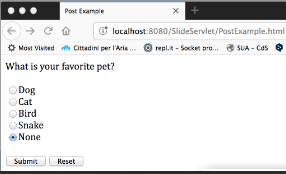
\includegraphics[scale=0.7]{img/form.png}
\end{center}
\subsection{Java Servlet}
Le \textbf{Java Servlets} sono piccole applicazioni Java residenti sul server, per esempio \textit{apache/Tomcat}. Una servlet è un componente gestito in modo automatico da un \textit{container} o \textit{engine} e ha un'interfaccia che definisce il set di metodi (ovviamente (ri)definibili). Si ha quindi maggior semplicità e standardizzazione ma magior rigidità del modello. Il container controlla le servlet (attiva/disattiva) in base alle richieste dei client. Inoltre le servelts sono residenti in memoria, mantengono uno stato (sono oggetti java) e consentono le interazioni tra di loro.\\
Si quindi la differenza tra \textbf{stateless} e \textbf{statefull}. HTTP non prevede persistenza, è quindi stateless e quindi non si possono mantenere informazioni tra un messaggio e i successivi e non si possono identificare i client. Si mantiene lo stato della conversazione con le servlet, con i cookies che sono informazioni memorizzate sul client che permettono di gestire le sessioni e con \textit{HTTPSession} che è gestito automaticamente dal container (con cookie o riscrittura delle URL).\\
Ogni servlet implementa l'interfaccia:
\begin{minted}{java}
javax.servlet.Servlet
\end{minted}
con 5 metodi:
\begin{minted}{java }
// init inizializza il server
void init(ServletConfig config) 

/* ServletContext restituisce i parametri di inizializzazione e 
il ServletContext che da accesso all’ambiente */
ServletConfig getServletConfig() 

// service è invocato per gestire le richieste dei client
void service(ServletRequest request, ServletResponse response) 

// getServletInfo restituisce informazioni tipo autore e versione 
String getServletInfo() 

/* la destroy è chiamata quando la servlet termina 
(es: per chiudere un file o una connessione con un database) */
void destroy()  
\end{minted}
L'interfaccia è solo la dichiarazione dei metodi che, per essere utilizzabili, devono essere implementati in una classe.\\
no presenti due classi astratte, cioé che implementano i metodi dell’interfaccia in modo che non facciano nulla. 
\begin{minted}{java}
javax.servlet.GenericServlet 

javax.servlet.http.HTTPServlet  /* che definisce 
                                   metodi per l'uso in ambiente web */
\end{minted}
Questo semplifica la scrittura delle servlet vere e proprie in quando basta implementare (ridefinendoli) solo i metodi che interessano.\\
Vediamo la classe \textit{HTTPServlet}. Questa classe implementa \textit{service} in modo da invocare i metodi per servire le richieste dal web. Si hanno:
\begin{itemize}
	\item \textit{doGet(), doHead(), doDelete(), doOptions(), doPost() e doTrace()} con i vari metodi HTTP
	\item due parametri: \textit{HTTPServletRequest e HTTPServletResponse}
	\item le eccezzioni: \textit{ServletException e IOException}
\end{itemize}
nche i parametri sono stati adattati al protocollo HTTP, cioè consentono di ricevere(inviare) messaggi HTTP leggendo(scrivendo) i dati nell'head e nel body di un messaggio. Si ha che:
\begin{itemize}
	\item all'interfaccia \textit{HTTPServletRequest} viene passato un oggetto da service, l'interfaccia contiene la richiesta del client e estende \textit{ServletRequest}
	\item all'interfaccia \textit{HTTPServletResponse} viene passato un oggetto da service, contiene la risposta per il client ed estende \textit{ServletResponse}
\end{itemize}
Vediamo i metodi principali:
\begin{minted}{java}
String getParameter(String name) /* Restituisce il valore
                                    dell’argomento name */

Enumeration getParameterNames() /* Restituisce l'elenco 
                                   dei nomi degli argomenti */

String[] getParametersValues(String name) /* Restituisce i valori 
                                             dell'argomento name */

Cookie[] getCockies() //Restituisce i cookies del server sul client 

void addCookie(Cookie cookie) /* Aggiunge un cookie
                               nell'intestazione della risposta  */

HTTPSession getSession(boolean create) /* Una HTTPSession
                                          identifica il client e 
                                          viene creata se create=true */
                                          
void setContentType(String type) /* Specifica il tipo MIME della
                                    risposta per dire al browser come 
                                    visualizzare la risposta 
                                    Es: “text/html” dice che è html */
                                          
ServletOutputStream getOutputStream() /* Restituisce lo stream di 
                                         byte per scrivere la risposta */

PrintWriter getWriter() /* Restituisce lo stream di 
                           caratteri per scrivere la risposta */ 
\end{minted}
qualche immagine:
\begin{center}
	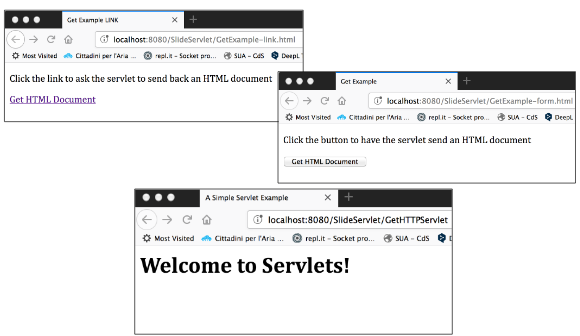
\includegraphics[scale=2.4]{img/servlet.png}
\end{center}
vediamo lato client una pagina HTMl con un URL alla risorsa servlet
\begin{minted}{html}
<DOCTYPEhtml>
<html>
<head>
<meta charset="UTF-8">
<title>GetExample LINK</title>
</head>
<body>
  <p>Click the link to ask the servlet to send back an HTML document</p>
  <a href="http://localhost:8080/SlideServlet/GetHTTPServlet"> 
  Get HTML document</a>
</body>
</html>
\end{minted}
vediamo nel caso del form, con il metodo di invio GET e la servlet che processa il form:
\begin{minted}{html}
<DOCTYPEhtml>
<html>
<head>
<metacharset="UTF-8">
<title>GetExample</title>
</head>
<body>

<form action="http://localhost:8080/SlideServlet/GetHTTPServlet"
      method="GET">
   <p>Click the link to ask the servlet to send back an HTML document</p>
   <input type="submit"value="Get HTML Document">
</form>
</body>
</html>
\end{minted}
\newpage
avendo lato server:
\begin{minted}{java}
// da Internet e WWW – How to program, Dietel&Dietel, Prentice Hall
// Creating and sending a page to the client

public classGetHTTPServletextendsHttpServlet {
  public void doGet(HttpServletRequest request,
                    HttpServletResponse response)
              throwsServletException, IOException {
     PrintWriter output;
     response.setContentType( "text/html" ); // contenttype
     output = response.getWriter(); // getwriter
     // create and send HTML page to client
     StringBufferbuf =new StringBuffer();
     buf.append( "<html><head><title>\n" );
     buf.append( "A Simple ServletExample\n" );
     buf.append( "</title></head><body>\n" );
     buf.append( "<H1>Welcome to Servlets!</H1>\n" );
     buf.append( "</body></html>" );
     output.println( buf.toString() );
     output.close();// closePrintWriterstream
  }
}
\end{minted}
vediamo un esempio lato server che converte Celsius e Fahrenheit:
\begin{center}
	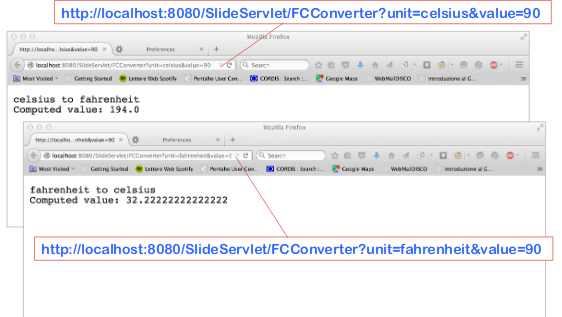
\includegraphics[scale=0.7]{img/cel.png}
\end{center}
\begin{minted}{java}
public class FCConverter extends HttpServlet {
  private String convertCtoF(Double celsius) {
    Double fahrenheit;
    fahrenheit = ((celsius * 9) / 5) + 32;
    return Double.toString(fahrenheit);
  }
  
  private String convertFtoC(Double fahrenheit) {    
    Double celsius;
    celsius = (fahrenheit - 32) * 5 / 9;
    return Double.toString(celsius);
  }
  
  protected void doGet(HttpServletRequest request,
                         HttpServletResponse response) 
                       throws ServletException, IOException {
    String result;     
    String unit=request.getParameter("unit");
    Double value = Double.parseDouble(request.getParameter("value"));
    
    if(unit.equals("fahrenheit")) {
      response.getWriter().append("fahrenheit to celsius \n");
      result=convertFtoC(value);
    } else {
      response.getWriter().append("celsius to fahrenheit \n");
      result = convertCtoF(value);
    }
    
    response.getWriter().append("Computed value: ").append(result);
  }
}   
\end{minted}
con i form:
\begin{center}
	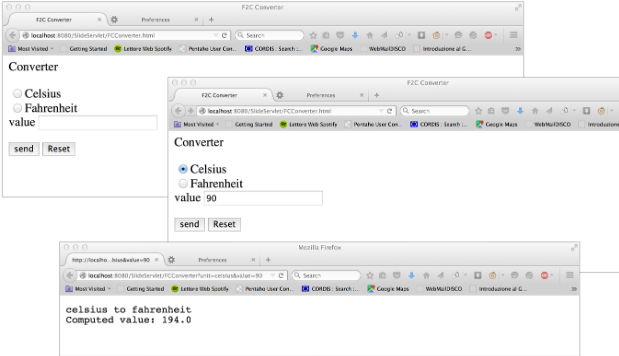
\includegraphics[scale=0.8]{img/cel3.png}
\end{center}
\begin{minted}{html}
<!DOCTYPEhtml> 
<html> 
<head>
<meta charset="UTF-8">
<title>F2C Converter</title>
</head>
<body>

<form action="http://localhost:8080/SlideServlet/FCConverter"
      method="GET">
   Converter <BR><BR>
   <input type="radio"name="unit"value="celsius">Celsius<BR>
   <input type="radio"name="unit"value="fahrenheit">Fahrenheit<BR>
   value <input type="text"name="value"><BR><BR>
   <input type="submit"value="send">
   <input type="reset">
</form>
</body>
</html>
\end{minted}
volendo anche una risposta HTML:
\begin{center}
	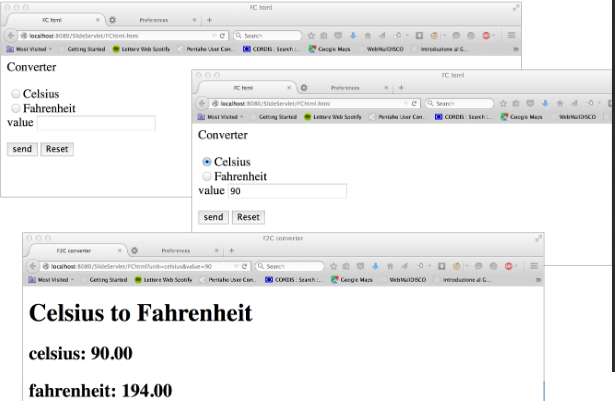
\includegraphics[scale=2.4]{img/cel4.png}
\end{center}
con la servlet:
\begin{minted}{java}
import java.io.IOException;
import java.text.DecimalFormat
import javax.servlet.ServletException;
import javax.servlet.annotation.WebServlet;
import javax.servlet.http.HttpServlet;
import javax.servlet.http.HttpServletRequest;
import javax.servlet.http.HttpServletResponse;

@WebServlet("/FChtml")
public class FCConverter extends HttpServlet {

  private Double convertCtoF(Double celsius) {
    Double fahrenheit;
    fahrenheit = ((celsius * 9) / 5) + 32;
    return fahrenheit;
  }
  
  private Double convertFtoC(Double fahrenheit) {    
    Double celsius;
    celsius = (fahrenheit - 32) * 5 / 9;
    return celsius;
  }
  
  protected void doGet(HttpServletRequest request,
                         HttpServletResponse response) 
                       throws ServletException, IOException {
    String unit=request.getParameter("unit");
    Double value = Double.parseDouble(request.getParameter("value"));
    Double result;    
    StringBuffer buf = new StringBuffer();
    
    buf.append( "<!DOCTYPE html>\n" );
    buf.append( "<html>\n<head>\n<title>F2C converter </title>\n</head>\n<body>\n" );
    if(unit.equals("fahrenheit")) {
      buf.append("<h1> Fahrenheit to Celsius </h1>\n");
      result=convertFtoC(value);
    } else {
      buf.append("<h1> Celsius to Fahrenheit </h1>\n");
      result=convertCtoF(value);
    }
    DecimalFormat twoDigits = new DecimalFormat( "#0.00" );
    buf.append("<h2>" + unit + ": " + twoDigits.format( value ) + "</h2>\n”);
    buf.append("<h2>");
    if( unit.equals("fahrenheit")) {
      buf.append("celsius: ");
    } else {
      buf.append("fahrenheit: ");
    }
    
    buf.append( twoDigits.format( result ) );
    buf.append( "</h2>\n" ); 
    buf.append( "</body>\n</html>" );
    response.getWriter().append(buf);
  }  
}    
\end{minted}
\newpage
Vediamo anche un esempio di POST:
\begin{center}
	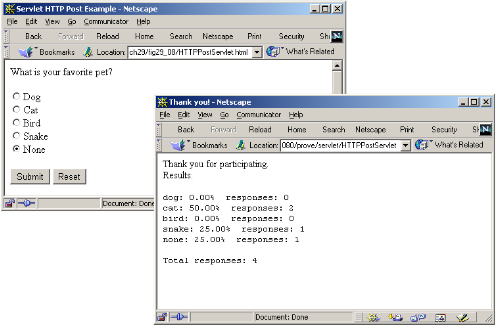
\includegraphics[scale=0.7]{img/post.png}
\end{center}
\begin{minted}{html}
<!DOCTYPE html>
<html>
<head>
<meta charset= "UTF-8" >
<title>Post Example</title>
</head>
<body>
  <form action= "http://localhost:8080/SlideServlet/PostHTTPServlet"
     method= "POST" >
     What is your favorite pet?<br>
     <br> <input type= "radio" name= "animal" value= "dog" >Dog<br>
     <input type= "radio" name= "animal" value= "cat" >Cat<br> <input
       type= "radio" name= "animal" value= "bird" >Bird<br> <input
       type= "radio" name= "animal" value= "snake" >Snake<br> <input
       type= "radio" name= "animal" value= "none" checked>None <br>
     <br>
     <input type= "submit" value= "Submit" > <input type= "reset" >
  </form>
</body>
</html> 
\end{minted}
con la seguente servlet lato server:
\begin{minted}{java}
public class HTTPPostServlet extends HttpServlet {
  // definisco l’elenco degli animali
  private String animalNames[] = {
    "dog",
    "cat",
    "bird",
    "snake",
    "none"
  };
  public void doPost(HttpServletRequest request,
    HttpServletResponse response)
  throws ServletException, IOException {
    int animals[] = null, // contatori di preferenze
      total = 0; // totale delle preferenze espresse
    // i dati sono memorizzati nel file "survey.dat"
    File f = new File("survey.dat"); // apro o creo il file
    if (f.exists()) { // leggo il file e lo assegno a animals
      animals = ...
        // conto quante sono le risposte date in precedenza
        for (int i = 0; i < animals.length; ++i)
          total += animals[i];
    } else // creo un nuovo array di contatori
      animals = new int[5];
    // leggo il messaggio con la nuova preferenza
    String value = request.getParameter("animal");
    ++total;
    // aggiorno il totale delle risposte
    // determino quello votato e aggiorno il suo contatore
    for (int i = 0; i < animalNames.length; ++i)
      if (value.equals(animalNames[i]))
        ++animals[i];
    // scrivo i nuovi contatori sul file e lo chiudo
    ObjectOutputStream output =
      new ObjectOutputStream(new FileOutputStream(f));
    output.writeObject(animals);
    output.flush();
    output.close();
    // calcolo le percentuali
    double percentages[] = new double[animals.length];
    for (int i = 0; i < percentages.length; ++i)
      percentages[i] = 100.0 * animals[i] / total;
    // costruisco l’head del messaggio di risposta
    response.setContentType("text/html"); // content type
    // predispongo alla scrittura del body del messaggio
    PrintWriter responseOutput = response.getWriter();
    // uso un Buffer di servizio per costruire la pagina
    StringBuffer buf = new StringBuffer();
    buf.append("<html>\n<title>Thank you!</title>\n");
    buf.append("Thank you for participating.\n");
    buf.append("<br>Results:\n<pre>");
    DecimalFormat twoDigits = new DecimalFormat("#0.00");
    for (int i = 0; i < percentages.length; ++i) {
      buf.append("<br>" + animalNames[i] + ": ");
      buf.append(twoDigits.format(percentages[i]));
      buf.append("% responses: " + animals[i] + "\n");
    }
    buf.append("\n<br><br>Total responses: " + total);
    buf.append("</pre>\n</html>");
    // scrivo la pagina nella risposta
    responseOutput.println(buf.toString());
  }
}
\end{minted}
Vediamo cosa succede quando si esegue una servlet. Si crea innanzitutto un'istanza della servlet, condivisa da tutti i client e ogni richiesta genera un Thread che esegue la \textit{do} appropriata. Una servlet viene creata dal container quando viene effettuata la prima chiamata. Viene invocato il metodo \textit{init()} per inizializzazioni specifiche e viene distrutta con \textit{destroy()} quando non ci sono servizi in esecuzione o in base ad un timer specifico. Container e richieste dei client devono sincronizzarsi sulla terminazione in quanto potrebbe esserci ancora in esecuzione la \textit{service()}, inoltre bisogna tener traccia dei thread in esecuzione, progettare il metodo \textit{destroy()} in modo da notificare lo
\textbf{shutdown} e attendere il completamento del metodo \textit{service()} e progettare i metodi lunghi in modo che verifichino periodicamente
se è in corso uno shutdown e comportarsi di conseguenza.
\subsection{Java JSP}
\textbf{Java Service Pages} (analogamente a ASP, \textit{Micorsoft Active Server Page} con VBScript e JScript) è una tecnologia per la creazione di applicazioni web. Specifica l'interazione tra un contenitore/server ed un insieme di "pagine" che presentano informazioni all’utente
Le pagine sono costituite da tag tradizionali (HTML, XML,
WML, ...) e da tag applicativi che controllano la generazione
del contenuto Rispetto ai servlet, facilitano la separazione tra logica applicativa e presentazione. Java Server Pages (JSP) separano la parte dinamica delle pagine dal template HTML statico e il codice si include dei tag <\% ... \%>.\\ Vediamo un esempio semplice, una pagina che visualizza "Grazie per la scelta di \textit{Internet Guida Pratica}" quando ci si connette ad  all'URL \textit{http://host/OrderConfirmation.jsp?title=Internet+Guida+Pratica}. La pagina conterrà:
\begin{minted}{html}
Grazie per la scelta di <i> <%= request.getParameter("title") %> </i>
\end{minted} 
La pagina viene convertita automaticamente in una servlet java la prima volta che viene richiesta.\\
Vediamo un altro esempio:
\begin{minted}{html}
<%@ page language="java" contentType="text/html; charset=UTF-8"
  pageEncoding="UTF-8"%>
<!DOCTYPE html PUBLIC "-//W3C//DTD HTML 4.01 Transitional//EN" "http://
www.w3.org/TR/html4/loose.dtd">
<html>
<head>
<meta http-equiv="Content-Type" content="text/html; charset=UTF-8">
<title>Welcome</title>
</head>
<body>
  <h1><%= ”Welcome to JSP!" %><h1>
</body>
</html>
\end{minted}
\begin{center}
	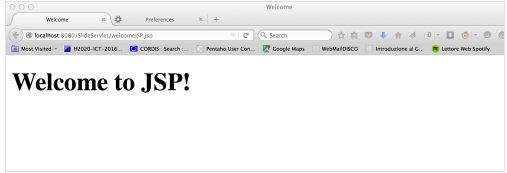
\includegraphics[scale=0.7]{img/jsp.png}
\end{center}
Vediamo gli elementi di una JSP:
\begin{itemize}
	\item \textbf{template text:} le parti statiche
	\item \textbf{commenti:} \textit{<\%-- questo e’ un commento -->}
	\item \textbf{direttive:} \textit{<\%@ direttiva ... di compilazione \%>}
	\item \textbf{azioni in XML:} \textit{<tag attributes> body </tag>}
	\item \textbf{elementi di scripting:}
	\begin{itemize}
		\item istruzioni nel linguaggio specificato nelle direttive
		\item sono di tre tipi: scriplet, declaration, expression
	\end{itemize}
\end{itemize}
Approfondiamo il discorso direttive. Si hanno:
\begin{itemize}
	\item \textbf{page:} sono liste di attributi/valori e valgono per la pagina dove sono inseriti:
	\begin{minted}{html}
    <%@ page import="java.util.*" buffer="16k" %>
    <%@ page import=“java.math.*, java.util.*” %>
    <%@ page session=“false” %>
	\end{minted}
	\item \textbf{include:} permette di includere in compilazione pagine HTML e JSP:
	\begin{minted}{html}
    <%@ include file="copyright.html" %>
	\end{minted}
	\item \textbf{taglib:} che dichiara tag definiti dall'utente implementando opportune classi:
	\begin{minted}{html}
    <%@ taglib uri=“TableTagLibrary” prefix=“table”%>
    <table:loop> ... </table:loop>
	\end{minted} 
\end{itemize}
Si hanno nello specifico delle direttive JSP:
\begin{itemize}
	\item \textbf{forward:} determina l'invio della richiesta corrente, eventualmente aggiornata con ulteriori parametri, all'URL indicata:
	\begin{minted}{html}
    <jsp:forward page=“login.jsp” %> 
      <jsp:param name=“username” value=“user” />
      <jsp:param name=“password” value=“pass” />
    </jsp:forward>
	\end{minted}
	\item \textbf{include:} invia dinamicamente la richiesta ad una data URL e ne include il risultato:
	\begin{minted}{html}
    <jsp:include page=“login.jsp” %>
	\end{minted}
	\newpage
	\item \textbf{useBean:} localizza ed istanzia (se necessario) un javaBean nel contesto specificato. Il contesto può essere:
	\begin{minted}{html}
     <jsp:useBean id=“cart” scope=“session” class=“ShoppingCart” />
	\end{minted}
\end{itemize}
Vediamo gli elementi di scripting:
\begin{itemize}
	\item \textbf{declaration:} della forma \textit{<\%! declaration [declaration] ...\%>} indicano le variabili e i metodi usati nella pagina e valgono per la durata della servlet:
	\begin{minted}{html}
    <%! int[] v= new int[10]; %>
	\end{minted}
	\item \textbf{expression:} della forma \textit{<\%= expression \%>}. Indica una espressione nel linguaggio di scripting che viene valutata e sostituita con il risultato:
	\begin{minted}{html}
    <p>La radice di 2 vale <%= Math.sqrt(2.0) %></p>
	\end{minted}
	\item \textbf{scriptlet:} della forma \textit{<\% codice \%>} sono frammenti di codice che controllano la generazione della pagina, valutati alla richiesta. Le variabili valgono per la singola esecuzione. Ciò che viene scritto sullo stream di output sostituisce lo scriptlet:
	\begin{minted}{html}
    <table>
    <% for (int i=0; i< v.length; i++) { %>
             <tr><td> <%= v[i] %></td></tr>
    <% } %>
    </table>
	\end{minted}
\end{itemize}
vediamo un esempio di uso di dati dinamici:
\begin{minted}{html}
<%@ page language="java" contentType="text/html;
    charset=UTF-8” pageEncoding="UTF-8"%>
<!DOCTYPE html PUBLIC "-//W3C//DTD HTML 4.01 Transitional//EN" 
  "http://www.w3.org/TR/html4/loose.dtd">
<html>
<head>
<meta http-equiv="Content-Type" content="text/html; charset=UTF-8">
<title>Uso di JSP</title>
</head>
<body BGCOLOR="#FDF5E6" TEXT="blue" >
<CENTER>
<TABLE BORDER=5 BGCOLOR="#EF8429">
  <TR><TH CLASS="TITLE">
    Using JavaServer Pages</TABLE>
</CENTER> <BR>
Some dynamic content created using various JSP mechanisms:
<UL>
  <LI><B>Expression.</B><BR>
    Your hostname: <%= request.getRemoteHost() %>.
  <LI><B>Scriptlet.</B><BR>
    <% out.println("Attached GET data: " + request.getQueryString()); %>
  <LI><B>Declaration (plus expression).</B><BR>
    <%! private int accessCount = 0; %>
    Accesses to page since server reboot: <%= ++accessCount %>
  <LI><B>Directive (plus expression).</B><BR>
    <%@ page import = "java.util.*" %>
    Current date: <%= new Date() %>
</UL>
</body>
</html>
\end{minted}
Un altro esempio:
\begin{minted}{html}
<%@ page language= "java" contentType= "text/html;
   charset=UTF-8" pageEncoding= "UTF-8" %>
<!DOCTYPE html PUBLIC "-//W3C//DTD HTML 4.01 
  Transitional//EN" "http://www.w3.org/TR/html4/loose.dtd">
<html>
<head>
<meta http-equiv= "Content-Type" content= "text/html; charset=UTF-8" >
<title>Uso di JSP</title>
<link rel= ”stylesheet" href= "My-Style-Sheet.css" type= "text/css” >
</head>
<body bgcolor= "#FDF5E6" text= "blue" >
  <center>
    <table border= "5" bgcolor= "#EF8429" >
      <tr>
        <th class= "title" > Using JavaServer Pages </th>
      </tr>
    </table>
  </center>
<br> Some dynamic content created using various JSP mechanisms:
<ul>
  <li><b>Expression.</b><br> Your hostname:
     <%=request.getRemoteHost()%>. </li>
  <li><b>Scriptlet.</b><br>
     <% out.println("Attached GET data: " +
        request.getQueryString()); %></li>
  <li><b>Declaration (plus expression).</b><br> 
    <%!private int accessCount = 0;%>
    Accesses to page since server reboot: 
    <%=++accessCount%> </li>
  <li><b>Directive (plus expression).</b><br>
    <%@ page import= "java.util.*" %> Current date: <%=new Date()%> </li>
  </ul>
</body>
</html> 
\end{minted}
ottenendo:
\begin{center}
	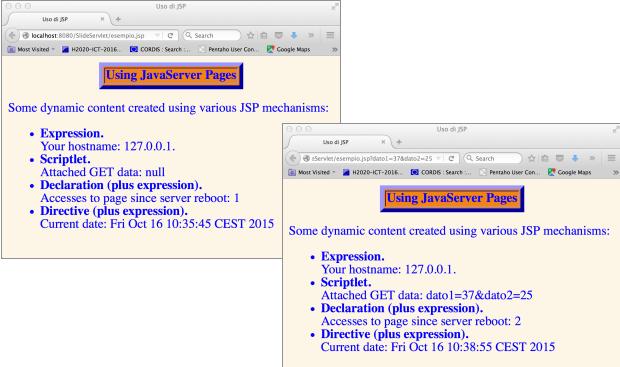
\includegraphics[scale=0.7]{img/jsp2.png}
\end{center}
vediamo un esempio di JSP con form HTML:
\begin{minted}{html}
<!DOCTYPE html>
<html>
<head>
<meta charset="UTF-8">
<title>JSP Example</title>
</head>
<body>
<form action="http://localhost:8080/SlideServlet/FC.jsp"
      method="GET"> 
  Converter <BR><BR>
  <input type="radio" name="unit" value="celsius">Celsius<BR>
  <input type="radio" name="unit"   value="fahrenheit">Fahrenheit<BR>
  value <input type="text" name="value" ><BR><BR>
  <input type="submit" value="send">
  <input type="reset">
</form>
</body>
</html>
\end{minted}
\begin{center}
	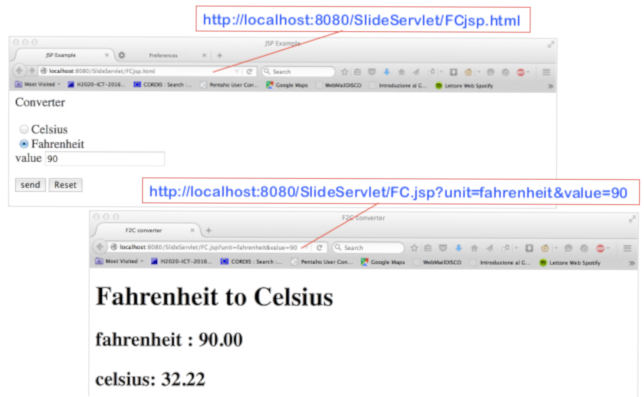
\includegraphics[scale=2.4]{img/jsp3.png}
\end{center}
\newpage
che in JSP diventa:
\begin{minted}{html}
<%@ page language="java" contentType="text/html; charset=UTF-8" pageEncoding="UTF-8"%>
<!DOCTYPE html PUBLIC "-//W3C//DTD HTML 4.01 Transitional//EN" 
  "http://www.w3.org/TR/html4/loose.dtd">
<html><head><meta http-equiv="Content-Type" 
  content="text/html; charset=UTF-8">
<title>F2C converter</title></head>
<body>
  <%@ page import = "java.text.DecimalFormat" %>
  <% Double result;
  String unit = request.getParameter("unit");
  Double value=Double.parseDouble(request.getParameter("value")); %>
  <h1> <% if( unit.equals("fahrenheit")) { %>
       <%= "Fahrenheit to Celsius" %>
       <% result=(value - 32)*5/9;
       } else { %>
       <%= "Celsius to Fahrenheit" %> 
       <% result=((value * 9) / 5) + 32; } %>
  </h1>
  <% DecimalFormat twoDigits = new DecimalFormat( "#0.00" ); %>
  <h2> <%= unit %> : <%= twoDigits.format(value) %> </h2>
  <h2> <% if( unit.equals("fahrenheit")) { %>
       <%= "Fahrenheit: " %>
       <% result=(value - 32)*5/9;
       } else { %>
       <%= "Celsius: " %>
       <% result=((value * 9) / 5) + 32; } %>
       <%= twoDigits.format( result ) %>
  </h2>
</body>
</html>
\end{minted}
\newpage
Vediamo gli elementi di scripting. Un linguaggio di scripting ha lo scopo di interagire con gli oggetti java e gestire le eccezioni java. SI hanno 9 oggetti impliciti, gli elementi delle servlet:
\begin{enumerate}
	\item requeste
	\item response
	\item out
	\item page
	\item pageContext
	\item session
	\item application
	\item config
	\item exception
\end{enumerate}
Gli oggetti possono essere creti in 3 modi:
\begin{enumerate}
	\item implicitamente usando le direttive JSP
	\item esplicitamente con le azioni
	\item direttamente usando uno script (raro)
\end{enumerate}
Gli oggetti hanno un attributo che ne definisce lo "scope":
\begin{center}
	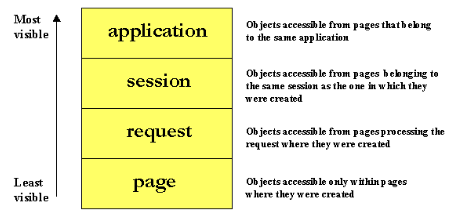
\includegraphics[scale=0.7]{img/scope.png}
\end{center}
che accede ad un oggetto HTTPSession. Per esempio si ha:
\begin{itemize}
	\item \textbf{memorizzazione}: 
	\begin{minted}{html}
    <% Foofoo = new Foo(); session.putValue("foo",foo); %>
	\end{minted}
	\item \textbf{recupero}:
	\begin{minted}{html}
    <% FoomyFoo = (Foo) session.getValue("foo"); %>
	\end{minted}
	\item \textbf{esclusione di una pagina dalla sessione}:
	\begin{minted}{html}
    <%@ page session="false" %>
	\end{minted}
\end{itemize}
Parliamo ora del \textbf{pattern Model View COntrol (\textit{MVC})} per la separazione tra dati, controllo e visualizzazione. Si ha che:
\begin{itemize}
	\item il client richiede via HTTP un file .JSP
	\item il file .JSP viene interpretato e accede a componenti lato-server (Java Beans, Servlet) che generano contenuti dinamici  
	\item il risultato viene spedito al client in forma di pagine HTML 
\end{itemize}
\begin{center}
	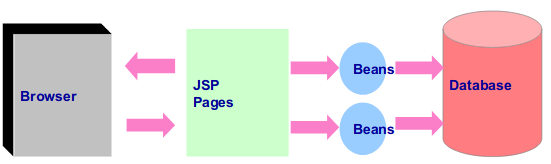
\includegraphics[scale=0.7]{img/mvc.png}
\end{center}
Un \textbf{bean} è una classe che segue regole precise:
\begin{itemize}
	\item ha un costruttore senza parametri
	\item dovrebbe avere campi (property) protetti \textit{private}
	\item i metodi di accesso ai campi (property) sono \textit{set e get}, quindi \textit{setXxx e getXxx/isXxx} (xxx = property) 
\end{itemize}
per esempio:
\begin{minted}{java}
class Book{
  private String title;
  private boolean available;
  void setTitle(String t) ...;
  String getTitle() ...;
  void setAvailable(boolean b) ...;
  boolean isAvailable () ...;
}
\end{minted}
Vediamo le azioni per utilizzare un bean:
\begin{itemize}
    \item \textbf{inizializzazione}, ovvero accedere ad un bin:
    \begin{minted}{html}
    jsp:useBean id="user" class="com.jguru.Person" scope="session" />
    <jsp:useBean id="user" class="com.jguru.Person" scope="session">
     <% user.setDate(DateFormat.getDateInstance( ).format(new Date())); 
       //etc.. %> 
    </jsp:useBean> 
    \end{minted}
    \item \textbf{accedere alle proprietà:}
    \begin{minted}{html}
    <jsp:getPropertyname="user" property="name" />
    <jsp:setPropertyname="user" property="name" value="jGuru" /
    ><jsp:setPropertyname="user" property="name" 
      value="<%=expression %>" />
    <jsp:useBean id="Attore" class="MyThread" scope="session"
      type="Thread"/>
    \end{minted}
\end{itemize}
Lo scope determina la vita di un bean e:
\begin{itemize}
    \item \textbf{page} è lo scope di default: viene messo in \textit{pageContext} ed acceduto con \textit{getAttribute}
    \item \textbf{request} viene messo in \textit{ServletReques}t ed acceduto con \textit{getAttribute}
    \item per \textbf{session \textit{e} application} si ha che se non esiste un bean con lo stesso id, ne viene creato uno nuovo
\end{itemize}
Inoltre si ha che il type permette di assegnare al bean una superclasse e che al posto della classe si può usare il nome del bean.\\
Vediamo un esempio di bean:
\begin{minted}{html}
<%@ page import= "itis.mvc.CounterBean" %>
  <jsp:useBean id= "session_counter" class= "itis.mvc.CounterBean"
    scope= "session" />
<jsp:useBean id= "app_counter" class= "itis.mvc.CounterBean"
  scope= "application" />
<%
  session_counter.increaseCount();
  synchronized (page) {
    app_counter.increaseCount();
  }
%>
<h3>
  Number of accesses within this session:
  <jsp:getProperty name= "session_counter" property= "count" />
</h3>
<p></p>
<h3>
  Total number of accesses:
  <%
  synchronized (page) {
  %>
  <jsp:getProperty name= "app_counter" property= "count" />
  <%
  }
  %>
</h3>
\end{minted} 
\begin{minted}{java}
public class CounterBean {
  //declare a integer for the counter
  private int count;
  
  public int getCount() {
    //return count
    return count;
  }
  public void increaseCount() {
    //increment count
    count++;
  }
}
\end{minted}
\begin{center}
	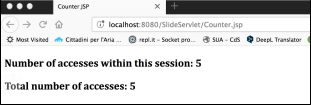
\includegraphics[scale=0.7]{img/count1.png}
\end{center}
\begin{center}
	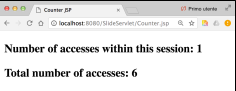
\includegraphics[scale=0.8]{img/count2.png}
\end{center}
\subsubsection{MVC2}
La richiesta viene inviata ad una Java Servlet che
\begin{itemize}
	\item genera i dati dinamici richiesti dall’utente
	\item li mette a disposizione della pagina jsp come Java “Beans”
\end{itemize}
e la servlet chiama una pagina .jsp che legge i dati del beans e organizza la presentazione in HTML che invia all'utente:
\begin{center}
	\includegraphics[scale=0.7]{img/mvc2.png}
\end{center}
L'MVC (\textit{Model View Control}) è formato da tre tipi di oggetti, che prima erano considerati un tutt'uno, incrementando così flessibilità e riutilizzo:
\begin{enumerate}
	\item il Model è \textbf{l'application object}
	\item il View e la \textbf{presentazione a schermo}
	\item il Controller è la componente che definire com l'interfaccia utente rispodne all'input
\end{enumerate}
\begin{center}
	\includegraphics[scale=0.7]{img/mvc22.png}
\end{center}
\chapter{HTML + CSS + JS}
Il linguaggio \textbf{HTML} è un linguaggio di markup, per dare struttura ai contenuti web,
utilizzato per annotare un documento in maniera tale che l'annotazione sia sintatticamente
distiguibile dal testo per diverse finalità:
\begin{itemize}
    \item di presentazione, in cui si definisce come visualizzare il testo al quale sono associate.
    \item procedurali, in cui si definiscono istruzioni per programmi che elaborino il testo associato.
    \item descrittive, in cui si etichettano semplicemente parti del testo, 
        al fine di disaccopiare la struttura dalla presentazione del testo spesso.
\end{itemize}
Un esempio di una pagina html si nota nella figura \ref{listato:htmlExample}

\begin{figure}
    \caption{Html example}
    \label{listato:htmlExample}
	\includegraphics[scale=0.9]{img/html.png}
\end{figure}
Il \textbf{CSS}(Cascading Style Sheets) è un linguaggio per dare uno stile ai contenuti web e la sua specifica
viene definita dal W3C(World Wide Web Consortium), un suo esempio si trova nella figura ~\ref{css:example}
mentre il DOM(Document Object Model) è un interfaccia neutrale rispetto al linguaggio e alla piattaforma
usata al fine di consentire l'accesso e la modifica dinamica di contenuto, struttura e lo stile di un
documento web, come si nota nella figura ~\ref{dom:example}.

\begin{figure}
    \caption{Css example}
    \label{css:example}
	\includegraphics[scale=0.9]{img/css.png}
\end{figure}

\begin{figure}
    \caption{Dom example}
    \label{dom:example}
	\includegraphics[scale=0.9]{img/dom.png}
\end{figure}
Ogni nodo può essere caratterizzato da attributi per facilitarne l'identificazione, la ricerca, la selezione:
\begin{itemize}
	\item un \textbf{identificatore univoco}, anche se il DOM non garantisce l'unicità
	\item una \textbf{classe} che indica l'appartenenza ad un insieme che ci è utile definire
\end{itemize}
Le \textbf{media query} possono essere viste come particolari selettori capaci di valutare le capacità
del device di accesso alla pagina (schermi, stamparti, text-to-speech), controllando le dimensioni
del device o della finestra, l'orientamento dello schermo e la risoluzione.
Vediamo un esempio:\\
\textit{se la pagina è più larga di 480
	pixel (e si sta visualizzando sullo schermo), applica
	determinati stili agli elementi con id "leftsidebar" (un menu) e "main" (la colonna centrale)}:
\begin{minted}{css}
@media screen and (min-width: 480px){
  #leftsidebar {width: 200px; float: left;}
  #main {margin-left:216px;}
}
\end{minted}
In CSS si ha il termine \textit{cascading} perché esistono potenzialmente diversi stylesheet:
\begin{itemize}
	\item l'autore della pagina in genere ne specifica uno (il modo più comunemente inteso) o più d'uno
	\item il browser ne ha uno, o un vero e proprio CSS o simulato nel loro codice
	\item il lettore, l’utente del browser, ne può definire uno proprio per customizzare la propria esperienza
\end{itemize}
Dei conflitti sono quindi inevitabili per cui è necessario definire un algoritmo per decidere quale
stile vada applicato a un elemento.\newline
Si ha il seguente ordine di importanza dei seguenti fattori associati alle regole:
\begin{enumerate}
	\item \textbf{importanza} (flag specifico \textit{!important} per un attributo)
	\item \textbf{specificità} (per esempio, \textit{id > class > tag})
	\item \textbf{ordine nel sorgente }(il più “recente” vince)
\end{enumerate}
Il browser non è solamente un banale visualizzatore di pagine scritte in HTML, è un vero e proprio 
ambiente di sviluppo (in particolare contiene un interprete Javascript e vari strumenti di debug,
ma ne parleremo più avanti) che fornisce numerose funzionalità abilitanti inoltre l'impostazione di
HTML e CSS separa nettamente il contenuto dalla modalità di visualizzazione.\newline
Esistono numerosi "front-end framework", dai più sofisticati ai più semplici, naturalmente open source, ad esempio:
\begin{itemize}
	\item \textbf{bootstrap}
	\item \textbf{foundation}
	\item \textbf{skeleton}
\end{itemize}

\subsection{HTML5}
HTML5 ha introdotto nuovi \textbf{elementi semantici} per la strutturazione delle pagine, per esempio:
\begin{itemize}
	\item article
	\item section
	\item aside
	\item header
	\item footer
\end{itemize}
Introduce inoltre nuovi \textbf{elementi di input e multimediali}, widget per input search, email,
url, number, tel, ma anche range, date \dots,  anche se il supporto a tutto ciò da parte dei browser non è uniforme.

L’HTML dovrebbe non contenere informazione di presentazione, riservata ai CSS, 
quindi senza stili definiti "in linea" e senza l'uso di tag come <font>, <b>, <i> ma dovrebbe solo 
occuparsi delle informazioni da volere rappresentare nel file web.

HTML5 sia più leggibile. In generale, a parte essere una notazione più concisa e che richiede
meno definizioni di classi, le gerarchie di contenuti più leggibili e analizzabili 
in fase di progettazione, manutenzione e debug.
\chapter{Web Service}
I \textbf{web services} stabiliscono un metodo per standardizzare la comunicazione, che viene basata
basata su documenti \textit{XML}. Questo sistema si basa sulla \textbf{SOA}, \textit{Software Oriented Architect}.
Un servizio offre servizi e funzionalità a clients indipendenti inoltre i servizi devono:
\begin{itemize}
\item fornire una descrizione per essere ndividuati e selezionati
\item devono fornire l'accesso mediante un protocollo noto
\item supportare la composizione per provvedere a soluzioni complesse
\item soddisfare i bisogni lato business del cliente e i requisiti di dominio 
\end{itemize}
Un \textbf{servizio} è \textit{un'entità software che può essere trovata e invocata da altri sistemi software}.
Il \textit{W3C} ci fornisce una definizione per \textbf{web service}:
\begin{center}
  \textit{Un web service è un'applicazione software identificata da un URI, con interfacce e binding
    (associazione interfaccia-protocollo-formato dei dati) che possono essere definiti descritti e scoperti da artefatti XML.
    Un web service supporta l'interazione diretta con altri software tramite lo scambio di
    messaggi XML tramite protocolli basati su Internet}
\end{center}
si possono avere altre due definizioni:
\begin{enumerate}
\item \textit{i web services sono applicazioni self-contained e self-described che possono essere pubblicate, localizzate e richiamate attaraverso il web}
\item \textit{le applicazioni web services sono componenti web incapsulate e debolmente accoppiate che possono collegarsi a vicenda dinamicamente}
\end{enumerate}
Si hanno le seguenti caratteristiche chiave:
\begin{itemize}
\item \textbf{software as service:} infatti sono distribuiti come flussi di servizi e permettono un accesso universale da qualsiasi piattaforma
\item \textbf{dynamic business interoperability:} infatti nuove partnership possono essere costruite dinamicamente e automaticamente dato che
  i web services assicurano una completa interoperabilità tra sistemi
\item \textbf{accessibility:} infatti i servizi internet possono essere decentralizzati, distribuiti in giro per il mondo e vi si può accedere con molti device
\item \textbf{efficiency:} infatti i business possono concentrarsi sui task cruciali e sul valore aggiunto dei loro prodotti, senza doversi concentrare
  sullo svlippo lento e costoso del software. I web services ostruiti da applicazioni per usi interni possono essere facilmente esposti per l'utilizzo esterno,
  permettendo uno sviluppo incrementale fondato su web services scritti in un linguaggio semplice anche da debuggare e fixare
\item \textbf{universally agreed specifications:} infatti i web services si basano su specifiche universali per scambio di dati, messaggi, scoperta di servizi,
  descrizione delle interfacce e orchestrazione dei processi business
\item \textbf{legacy integration:} infatti si ha una grande agilità e flessibilità dall'incrementare l'integrazione di sistemi legacy
\item \textbf{new market opportunity:} infatti la grande dinamicità dei web services si adatta facilmente al dinamismo del business
\item l'\textbf{indipendenza dei web services}, infatti sono \textit{componenti indipendenti} con:
  \begin{itemize}
  \item un'\textbf{interfaccia nota}, dotata di un linguaggio di descrizione standard (es. WSDL)e di una possibile gestione automatica da parte del middleware
  \item un \textbf{punto di accesso unico}, caratterizzato dall'uso di URI (URL/URL) e dal possibile sviluppo di name services (es. UDDI)
  \item lo \textbf{scambio di dati basato su messaggi}, con l'uso di un formato standard (es. XML), superando il classico scambio di parametri
  \end{itemize}
\end{itemize}
I web services sono consistenti con i principi della SOA dove si hanno:
\begin{itemize}
\item i \textbf{web service component} ovvero \textit{service} e \textit{service descriptor}
\item i \textbf{web service roles} ovvero \textit{service provider}, \textit{service brokers} \textit{service requestors}
\item le \textbf{web services operations} ovvero \textit{publish}, \textit{find} e \textit{interact}
\end{itemize}
\begin{center}
\includegraphics[scale=1]{img/soa.png}
\end{center}
si hanno le seguenti peculiarità dei web services:
\begin{itemize}
\item componenti pubblici ("scopribili", interfacce pubbliche)
\item componibilità (orchestrazione e coreografia di servizi composti e coordinati)
\item descrizioni semantiche (scoperta, composizione, raccomandazione di servizi, ...)
\item QoS (sicurezza, disponibilità, performance, context awareness)
\item organizzazione dei sistemi:
  \begin{itemize}
    \item p2p (application managed)
    \item ESB (middleware managed)
    \item grid (given model)
  \end{itemize}
\end{itemize}
e i seguenti problemi:
\begin{itemize}
\item descrizione funzionale e QoS
\item composizione, orchestrazione, coreografia
\item emantica
\item infrastruttura (naming, gestione dei servizi, ...)
\item ingegneria del software (sviluppo e deploy)
\item servizi per servizi (servizio di scoperta globale, reputazione, sicurezza, ...)
\item business (modelli economici e di organizzazione, processi, ...)
\end{itemize}
Vediamo una definizione per \textbf{web semantic}: \textit{il web semantic è un'estensione del web attuale nel quale l'informazione
  è fornita con un significato ben definito, permettendo una migliore cooperazione tra computer e persone}\\
Si ha quindi:
\begin{itemize}
\item cooperazione fra siti web, risorse e servizi per lo scambio di documenti e informazioni
\item l'uso di linguaggi semantici, per l'ontologia e per ``intelligent agents'':
  \begin{itemize}
  \item RDF: Resource Description Framework
  \item OWL: Web Ontology Language
  \end{itemize}
\item lo sviluppo di metaservizi per supportare la scoperta di servizi come:
  \begin{itemize}
  \item registri di metadati (ovvero descrizioni semantiche ricercabili)
  \item matchmaking (ovvero servizi che forniscono la corretta risposta ad una richiesta dell'utente)
  \end{itemize}
\end{itemize}
Analizziamo ora lo \textbf{XaaS stack}:
\begin{center}
\includegraphics[scale=0.35]{img/xaas.png}
\end{center}
\newpage
parte della \textbf{cloud computer architecture}:
\begin{center}
\includegraphics[scale=0.7]{img/cloud.png}
\end{center}
analizziamo ora le tre categorie di servizi:
\begin{enumerate}
\item \textbf{Software delivery model, SaaS (Software as a Service)} che fornisce all'utente un'applicazione software completa.
  Il cloud service provider gestisce l'infrastruttura cloud (servers, network, operating systems, storage and application software)
  lasciando ignaro l'utente di questo processo. Si fornisce un'interfaccia utente semplice e multipiattaforma, accessibile universalmente
  \begin{center}
  \includegraphics[scale=0.7]{img/saas.png}
  \end{center}
\item \textbf{Platform delivery model, Paas (Platform as a Service)} che fornisce
  all'utente gli strumenti per sviluppare e fare il deploy di applicazioni sul cloud
  usando i developer tools, le APIs e librerie software fornite dal provider del cloud. Il cloud service provider gestisce l'infrastruttura cloud (servers, network, operating systems, storage and application software) mentre l'utente sviluppa e deploya
\begin{center}
\includegraphics[scale=0.7]{img/paas.png}
\end{center}
\item \textbf{Infrastructure delivery model, IaaS (Infrastructure as a Service)}
  che fornisce all'utente di occuparsi delle risorse di memoria e computazione sonotto forma di macchine virtuali gestite dall'utente mentre il provider del cloud gestisce l'infrastruttura.
  Si ha il paradigma  \textit{pay-per-use/pay-as-you-go}:
  \begin{center}
\includegraphics[scale=0.7]{img/iaas.png}
\end{center}
\end{enumerate}
\subsection{Web Services Composition}
Si hanno innanzitutto i \textbf{business processes}, \textit{un insieme di attività logicamente collegate per raggiungere un obiettivo ben definito}:
\begin{itemize}
\item può prevedere particolari output al completamento e l'avvio a particolari condizioni
\item può includere interazione fra i partecipanti
\item durata variabile, in genere long term
\item varie attività manuali e/o automatiche
\item distribuito e personalizzato per le varie aziende
\item solitamente una singola istanza viene eseguita per mesi o anni
\end{itemize}
Un \textbf{workflow} è \textit{una sequenza di step a cui sono sottoposti oggetti fisici e informazioni. Includono attività, punti di decisione, varie strade, regole, ruoli.}\\
I service provider offrono le funzionalità che un workflow richiede dai business partner in un processo business. 
I service provider forniscono un'interfaccia pubblica in formato WSDL e la composizione del web service consiste
in un insieme di servizi interconnessi che a sua volta può essere usato come nuovo servizio in un'altra composizione.
Le operazioni devono essere compatibili per garantire il successo della composizione di servizi.\\
si definiscono anche:
\begin{itemize}
\item \textbf{orchestrazione:} che descrive come i web services possono interagire traloro a livello messaggi,
  includendo la logica business e l'ordine di esecuzione delle interazione sotto il
  controllo di un singolo endpoint
\item \textbf{coreografia:} che descrive la sequenze dei messaggi che possono coinvolgere più parti. Definisce lo lo stato condiviso delle interazioni fra businesses
\end{itemize}
\begin{center}
  \includegraphics[scale=0.6]{img/ws1.png}
\end{center}
\begin{center}
  \includegraphics[scale=0.7]{img/ws2.png}
\end{center}
\begin{center}
  \includegraphics[scale=0.5]{img/ws3.png}
\end{center}
\newpage
\subsection{WSDL}
È il \textit{Web Service Description Language} e indica dove e come accedere al servizio.
È un linguaggio basato su XML usato per descrivere i web services e come accederci.
WSDL è simile a Java Interfaces o CORBA IDL.\\
WSDL, che è raccomandato dal W3C, descrive 4 pezzi critici di dati:
\begin{enumerate}
\item informazioni sull'interfaccia che descrive tutte le operazioni disponibili pubblicamente
\item dichiarazione dei tipi di dato per tutti i messaggi di richiesta e risposta
\item informazione sul binding a livello di trasporto
\item informazioni sull'addressing per localizzare il servizio
\end{enumerate}
Il modello concettuale del WSDL 2.0 si divide in due parti:
\begin{enumerate}
\item \textbf{parte astratta:} che consiste in:
 \begin{itemize}
 \item una descrizione di un web service in termini di messaggi che manda/riceve attraverso (tipicamente tipizzati secondo W3C XML Schema)
 \item dei patterns di scambio di messaggi che definiscono sequenza e cardinalità dei messaggi
 \item un'operazione che associa un pattern di scambio di messaggi a uno o più messaggi
 \item un'interfaccia che raccoglie le operazioni in un formato per il trasporto
 \end{itemize}
\item \textbf{parte concreta:} che consiste in:
  \begin{itemize}
    \item i binding specificano il formato di trasporto delle interfacce
    \item l'endpoint di un servizio associa indirizzi network con un binding   
   \item un servizio raggruppa gli endpoint che implementano un'interfaccia comune
  \end{itemize}
\end{enumerate}
\begin{center}
\includegraphics[scale=0.7]{img/wsdl.png}
\end{center}
Si hanno 4 tipi di operazioni WSDL:
\begin{enumerate}
\item \textbf{one-way}: operazione riceve un messaggio e non risponde
\item \textbf{request-response}: operazione riceve una richiesta e risponde
\item \textbf{solicit-response}: operazione può mandare una richiesta e attende una risposta
\item \textbf{notification}: operazione può mandare una richiesta e non attende una risposta
\end{enumerate}
e si hanno delle regole per la propagazione dei fallimenti in merito a:
\begin{itemize}
\item \textbf{gestione dei fallimenti:}
  \begin{itemize}
    \item WSDL specifica la propagazione dei fallimenti, non la loro generazione
    \item la propagazione è definita come il tentativo best effort di trasmettere il messaggio di errore al giusto destinatario
    \item la generazione di un fallimento termina lo scambio
    \item binindings, feautures etc potrebbero sovrascrivvere la semantica di una propagazione degli errori ma è una procedura \textbf{fortemente sconsigliata} 
  \end{itemize}
\item \textbf{un fallimento che sostituisce un messaggio:}
  \begin{itemize}
    \item qualsiasi messaggio dopo il primo del pattern può essere sostituito con un messaggio di fallimento, che deve avere la stessa
      direzione e lo stesso nodo destinatario del messaggio che sostituisce
    \item se non c'è un modo di arrivare al destinatario, il fault viene scartato
  \end{itemize}
\item \textbf{un messaggio che scatena l'errore:}
  \begin{itemize}
    \item qualsiasi messaggio, primo incluso, può scatenare un messaggio di fallimento in risposta
    \item ogni destinatario può propagare l'errore e deve propagare al massimo un fallimento per messaggio di errore
    \item la direzione del messaggio di errore è l'inversa di quella del messaggio di arrivo
    \item il messaggio di errore deve essere mandato a colui che ha mandato il messaggio che ha scatenato l'errore
    \item se non c'è un modo di arrivare al destinatario, il fault viene scartato
  \end{itemize}
\item \textbf{nessun fallimento:} dove nessun errore deve essere propagato
\end{itemize}
\begin{center}
\includegraphics[scale=0.7]{img/fault.png}
\end{center}
\begin{shaded}
\begin{center}
\includegraphics[scale=2.3]{img/wsdl2.png}
\end{center}
\begin{center}
\includegraphics[scale=0.6]{img/wsdl3.png}
\end{center}
\begin{center}
\includegraphics[scale=0.6]{img/wsdl4.png}
\end{center}
\begin{center}
\includegraphics[scale=2.3]{img/wsdl5.png}
\end{center}
\begin{center}
\includegraphics[scale=0.6]{img/wsdl6.png}
\end{center}
\end{shaded}
\subsection{SOAP}
\textbf{SOAP} protocollo basato su XML per consentire a componenti software e applicazioni di comunicare tramite protocolli internet
standard (HTTP, SMTP, ...). Inoltre:
\begin{itemize}
\item è stateless
\item è one-way (richiesta/risposta, può passare per intermediari, no multicast)
\item ignora la semantica dei messaggi scambiati
\item l'effettiva interazione deve essere scritta nel documento SOAP
\item ogni pattern di comunicazione deve essere implementato dai sistemi sottostanti
\end{itemize}
provvede un modo standard di strutturare messaggi XML:
\begin{itemize}
\item applicazione delle specifiche XML
\item si affida a XML Schema e XML Namespaces
\end{itemize}
Inoltre è legato da linguaggi/piattaforme, è semplice e estensibile, passa dati strutturati e tipizzati.\\
Serve ad accedere a registri ed invocare servizi. Inoltre sono gli endpoint a definire la semantica.\\
Vediamo le componenti di un \textbf{messaggio SOAP}:
\begin{itemize}
\item \textbf{SOAP envelope} che definisce contenuti messaggio (cos'è, a chi è indirizzato, se è opzionale/obbligatorio)
\item \textbf{SOAP header (\textit{opzionale})} che presenta le seguenti caratteristiche:
  \begin{itemize}
    \item flessibile, può essere processato dai nodi intermediari
    \item contiene informazioni su come processare il messaggio: routing, impostazioni d'invio, autorizzazioni, transazioni ...
    \end{itemize}
\item \textbf{SOAP body} che è il messaggio effettivo che viene consegnato e processato. Contiene informazioni su chiamate e risposte
\end{itemize}
\begin{center}
\includegraphics[scale=0.6]{img/soap.png}
\end{center}
\section{RESTful Web Services}
Vediamo innanzitutto un paragone tra REST e SOAP:
\begin{center}
\includegraphics[scale=0.6]{img/rest.png}
\end{center}
e vediamo le varie differenze:
\begin{center}
\includegraphics[scale=0.6]{img/rest2.png}
\end{center}
e si ha lo \textbf{XaaS (Everything as a Service):}
\begin{center}
\includegraphics[scale=0.6]{img/xaas2.png}
\end{center}
La maggior parte dei servixi fornisce Web APIs. Si ha l'uso delle chiamate di procedura HTTP a tunnel (?) inoltre operazioni e dati hanno una semantica sconosciuta. \\
I sistemi distribuiti devono essere basati su un modello condiviso. WSDL/SOAP sono sistemi tradizionali che devono concordare sull'uso di API comuni. Inoltre i sistemi WSDL/SOAP SOA devono concordare su diversi messaggi.\\
REST semplifica questi accordi:
\begin{itemize}
\item i sostantivi sono necessari per nominare le risorse di cui si può parlare
\item i verbi sono le operazioni che possono essere applicate alle risorse nominate
\item i tipi di contenuto definiscono quali rappresentazioni di informazioni sono disponibili
\end{itemize}
REST (REpresentational State Transfer) è uno stile architetturale(una definizione di ruoli e funzionalità che permette di relazionare gli elementi) per sistemi distribuiti. Si ha che:
\begin{itemize}
\item le risorse sono definite da URI
\item le risorse sono manipolate tramite rappresentazioni (desiderate: campo Accept; restituite: campo Content-Type; specificate con MIME)
\item ci sono più rappresentazioni per una risorsa
\item si hanno messaggi autodescrittivi e stateless
\item lo stato dell'applicazione è guidato dalla manipolazione di risorse
\item si ha l'hypermedia per controllare il comportamento dell'applicazione:
  \begin{itemize}
    \item transizioni di stato del client avvengono tramite links
    \item link determinati e forniti dal server
  \end{itemize}
\item i principi REST si addicono ai componenti architetturali del web: URI e HTTP ( si usano quindi GET, POST, DELETE, PUT, HEAD, OPTIONS di HTTP)
\end{itemize}
Inoltre il client mantiene lo stato attraverso i link essendo stateless.\\
Si hanno diversi vantaggi:
\begin{itemize}
\item è scalabile
\item si ha un basso accoppiamento tra le risorse: no informazioni di sessione condivise
\item il caching migliora le prestazioni
\item il load balancing è più facile perché si hanno meno stati di comunicazione
\item è semplice perché si ha  meno software specializzato
\item si ha l'identificazione tramite meccanismi standard
\item si ha un uso completo e corretto protocollo HTTP
\item si ha un meccanismo leggero e stratificato per integrazione di dati e servizi
\item si ha una piattaforma distribuita e guidata dagli hypermedia
\end{itemize}
Se un sistema rispetta tutti questi vinoli è RESTful, altrimenti può essere più o meno RESTful. Inoltre:
\begin{center}
\textit{REST is not a set of laws or even a specification. It’s a style!}
\end{center}
Si ha l'astrazione delle informazioni chiave, mediante le risorse. Una risorsa è una qualsiasi informazione che può essere definita
mediante un nome (documenti, immagini ...). Le risorse hanno uno stato che può cambiare nel tempo. Inoltre hanno degli identificatori ed
espongono un'interfaccia semplificata, semplificando l'architettura e incoraggiando l'indipendenza delle implementazioni;
questi ultimi due aspetti, identificatori e semplificazione, sono dei vincoli. Quando si ha una richiesta può avvenire il trasferimento,
mediante una risorsa, dello stato al client; si richiede quindi il vincolo di avere un'architettura \textit{client-server}. A sua volta il client può
trasferire una proposizione di rappresentazione della risorsa stessa; si ha quindi il vincolo della manipolazione delle risorse mediante rappresentazione.
Infine la rappresentazione ritornata dal server può linkare ad uno stato aggiuntivo dell'applicazione. Il client può quindi seguire il link
e assumere il nuovo stato; si ha il vincolo dell'uso dell'hypermedia come engine per lo stato delle applicazioni.\\
Si ha poi il vincolo delle interazioni stateless che comporta che ogni interazione tra client e server contenga tutte le informazioni
necessarie a comprendere la richiesta e non sfrutta nessun dato salvato sul server. Si necessitano quindi messaggi auto-descrittivi,
con formati media standardizzati e con l'uso di \textit{meta-data} e\textit{control-data}. Si ottiene quindi un sistema \textit{cacheable} che però richiede un
sistemastratificato.
\newpage
Vediamo uno schema riassuntivo:
\begin{center}
\includegraphics[scale=0.7]{img/cont.png}
\end{center}
Tutti questi vincoli servono a fronteggiare gli otto errori della programmazione di rete:
\begin{enumerate}
\item la rete è sicura
\item la altenza è nulla
\item la banda è infinita
\item la rete è affidabile
\item la topologia non cambia
\item c'è un solo amministratore
\item il trasporto è privo di costi
\item la rete è omogenea
\end{enumerate}
\textbf{Un sistema distribuito privo di vincoli sarebbe inutile e ingestibile}\\
D'altro canto REST è un insieme di vincoli architetturali con lo scopo di minimizzare la latenza massimizzando indipendenza e scalabilità.
REST permette il caching, il riutilizzo delle interazioni, la sostituzione dinamica delle componenti e la computabilità delle azioni da parte di intermiediari,
in accordo coi biosgni del sistema a hypermedia.\\
REST punta quindi sulla semplicità:
\begin{itemize}
\item il caching aumenta le performance in risposta e riduce il carico sul server
\item meno stati di comunicazione permettono di meglio bilanciare il carico tra i server
\item meno software specializzato grazie alla presenza di software semplice alla base
\item l'identificazione viene fatto mediante meccanismi standard, senza nominazioni aggiuntive
\end{itemize}
inoltre REST è standard, quindi:
\begin{itemize}
\item si ha un uso corretto e completo del protocollo HTTP
\item si fornisce un meccanismo leggero e stratificato per l'integrazione di dati e servizi sopra HTTP
\item grazie ad HTTp si fornisce una piattaforma distribuita e gestita mediante hypermedia
\end{itemize}
\subsection{HTTP e REST Applications}
Si hanno 4 step:
\begin{enumerate}
\item \textbf{trovare tutti i nomi}. Ogni cosa in un sistema RESTful è una risorsa, con un nome. Ogni risorsa ha un URI che deve essere descrittivo
  e ben formato (sia semanticamente che sintatticamente, in modo che non serva cambiarlo nel tempo). Si usano le variabili PATH per gestire la gerarchia
  (padre/figlio) e la punteggiatura (``;'', ``,'') per la gerarchia implcita. Si hanno delle varibili di query (``?'') per indicare un input. Inoltre, per quanto un URI
  possa essere lungo a piacere si preferisce una lunghezza sensata. È buona norma non specificare informazioni sulla piattafroma in uso (tipo il linguaggio di prpgrammazione)
  nell'URI. \newpage Vediamo un esempio:
  \begin{center}
    \includegraphics[scale=0.7]{img/nouns.png}
  \end{center}
\item \textbf{definire il formato}. Si possono avere varie rappresentazioni, come XML e JSON, e se ne permette la creazione di nuove. Il formato in entrata deve però essere
  uguale al formato in uscita, con il client che può effettuare una GET, fare modifiche, fare una PUT... e il server che deve scartare ogni dato estraneo.
  Un media-type utile per il business è l'XHTML, che ha i vantaggi dell'XML con una maggiore accessibilità, con classi etc... che forniscono valori
  dotati della semantica necessaria (si usa \textit{<amount>1000.00</amount>} al posto di \textit{<span class="amount">1000.00</span>}).\\
  \textit{approfondimento a riguardo su XHTML sulle slide}
\item \textbf{scelta delle operazioni}. Sulle risorse possono essere effettuate varie operazioni; solitamente basta il set di operazioni di HTTP:
  \begin{itemize}
  \item GET, per recuperare una risorsa (non si devono avere effetti collaterali)
  \item POST, per aggiungere qualcosa ad una risorsa esistente sul server, che sceglie l'URI
  \item PUT, per caricare una risorsa sul server, il client sceglie l'URI
  \item DELETE, per eliminare una risorsa
  \end{itemize}
  inoltre si hanno altre operazioni non essenziali, come TRACE e CONNECT, altre non supportare universalmente, come OPTIONS, oltre ad operazioni come HEAD.\\
  \begin{center}
    \includegraphics[scale=0.6]{img/app1.png}
  \end{center}
  \begin{center}
    \includegraphics[scale=0.6]{img/app2.png}
  \end{center}
\item \textbf{evidenziare codici di stato}. Si hanno dei codici a 3 cifre per il risultato di una request:
  \begin{itemize}
  \item \textit{1xx (informational):} indica che la richiesta è stata ricevuta e che il server continua a lavorare
  \item \textit{2xx (success):} indica che la richiesta è stata ricevuta, compresa, accettata ed elaborata
  \item \textit{3xx (redirection):} indica che ulteriori azioni devono essere intraprese per completare la richiesta
  \item \textit{4xx (client error):} indica che la richiesta contiene errori di sintassi e non può essere elaborata
  \item \textit{5xx (server error):} indica che il server non è riuscito ad elaborare una richiesta apparentemente ben formata
  \end{itemize}
\end{enumerate}
Un client può richiedere una particolare rappresentazione (XML, JSON...) attraverso un header di richiesta, per esempio:
\begin{verbatim}
Accept: text/xml,application/xml,application/xhtml+xml,
text/html;q=0.9,text/plain;q=0.8,image/png,*/*;q=0.5
Accept-Language: en-us,en;q=0.5
Accept-Encoding: gzip,deflate
Accept-Charset: ISO-8859-1,utf-8;q=0.7,*;q=0.7 q = relative preference (0-1)
\end{verbatim}
Nella realtà non funziona così però e si preferisce esporre il tipo nell'uri:
\begin{verbatim}
http://expenses.example.com/123.xml
http://expenses.example.com/123.xhtml
http://expenses.example.com/123.json
Dots preferred over slashes: http://expenses.example.com/123/xml
\end{verbatim}
Si possono avere dei \textit{conditional GET}, salvando banda e quantità di dati da processare sia lato client che server:
\begin{center}
\includegraphics[scale=0.7]{img/condget.png}
\end{center}
COme abbiamo già indicato si ha il caching per ridurre latenza e traffico. Solo le GET (non-SSL) lo supportano. Si hanno due tipi:
\begin{enumerate}
\item \textbf{browser (user agent)}
\item \textbf{proxy}, i siti più grandi usano dei \textit{caching proxy server}
\end{enumerate}
\newpage
L'applicazione deve sapere dove sia del contenuto in cache e si hanno degli appositi cache-headers:
\begin{center}
  \includegraphics[scale=0.7]{img/cachehead.png}
\end{center}
\subsection{REST Services e RESTful Services}
Molte applicazioni REST attuali sono reimplementazioni di applicazioni CRUD (\textit{Create, Read, Update, Delete}), dove mancava l'hypermedia-control:
\begin{center}
\includegraphics[scale=0.6]{img/crud.png}
\end{center}
\begin{center}
\includegraphics[scale=2.0]{img/crud2.png}
\end{center}
Nel caso \textbf{statelessness} si ha che ogni richiesta avviene in modo isolato.
Il client mantiene lo stato dell'applicazione, tutte le risorse sono nella richiesta
e il server non usa nulla delle richieste precedenti. \textit{Gli stati possibili di un server sono risorse con URI}.\\
Si ha l'eliminazione di molte condizioni di errore in cui i clienti possono eseguire
operazioni non permesse.\\
Le applicazioni stateless sono bilanciate a livello di carico, partizionate, scalate e dotate di cache. Si ha una maggior possibilità di evitare danni irreversibili e si evitano
le sessioni (che compoterebbero messaggi non autodescrittivi etc...).\\
I server dovrebbero dimenticarsi dei client tra una richiesta e l'altra (no cookies).\\
Si ha il concetto di \textbf{HATEOAS}, \textit{Hypermedia As The Engine Of Application state}.
Dove lo stato dell'applicazione viene mantenuto dal client mentre il server mantiene
lo stato della risorsa. COme hypermedia si usano link e form e seguire un link, fornito dal server in un hypertext, è un passaggio di stato.
\begin{center}
\includegraphics[scale=2.3]{img/hy.png}
\end{center}
\begin{center}
\includegraphics[scale=0.7]{img/bho.png}
\end{center}
\chapter{Remote Procedure Call}
Le \textit{Remote Procedure Call (RPC)} sono una estensione al distribuito del normale
protocollo di chiamata di procedura e hanno diversi pro e contro:
\begin{itemize}
\item \textbf{pro:}
  \begin{itemize}
    \item hanno una semantica nota: chiamata di procedura
    \item sono facili da implementare: vicine al modello client-server
  \end{itemize}
\item \textbf{contro:}
  \begin{itemize}
    \item realizzate dal programmatore: tutto è esplicito
      [si può ovviare usando modelli a componenti più sofisticati]
    \item sono statiche: scritte nel codice dei programmi
      [si può ovviare usando chiamate indirette]
    \item non c’è concorrenza: sono bloccanti
      [si può ovviare con un uso appropriato dei thread o chiamate asincrone]
  \end{itemize}
\end{itemize}
Il modello RPC maschera il modello client-server:
\begin{center}
\includegraphics[scale=o.7]{img/rpc.png}
\end{center}
che si differenzia nel caso di RPC asincrono:
\begin{center}
\includegraphics[scale=0.7]{img/rpc2.png}
\end{center}
o dal caso in cui si hanno due rpc asincroni:
\begin{center}
\includegraphics[scale=0.7]{img/rpc3.png}
\end{center}
Analizziamo meglio l'architettura RPC. Si usano degli \textit{stub}. Stub o anche metodo stub, è una porzione di codice utilizzata in sostituzione di
altre funzionalità software in quanto può simulare il comportamento di codice
esistente (come una routine su un sistema remoto) o l'interfaccia COM
(Component Object Model (noto con l'acronimo COM, inglese per Modello a oggetti
per componenti) è un'interfaccia per componenti software),
e temporaneo sostituto di codice ancora da sviluppare.\\
Gli stub si usano per:
\begin{itemize}
\item simulare comportamenti locali per chiamante e chiamato
\item realizzare la comunicazione tra processi remoti
\end{itemize}
\begin{center}
\includegraphics[scale=2.3]{img/stub.png}
\end{center}
Si ha il passaggio di parametri per valore:
\begin{center}
\includegraphics[scale=0.7]{img/stub2.png}
\end{center}
Quindi tutti i dati vengono ``impacchettati'', spediti,
``spacchettati'' e riprodotti e si ha il \textit{marshalling/unmarshalling} dei dati:
\begin{center}
\includegraphics[scale=0.7]{img/stub3.png}
\end{center}
nel complesso ecco l'esecuzione di una RPC:
\begin{center}
\includegraphics[scale=0.7]{img/rpct.png}
\end{center}
\section{RMI}
Vediamo un'immagine introduttiva sull'architettura di riferimento, basata su oggetti distribuiti:
\begin{center}
\includegraphics[scale=0.7]{img/rmi.png}
\end{center}
Si hanno:
\begin{itemize}
\item \textbf{oggetti}, che incapsulano i dati (lo stato) mediante i valori dei
  campi e delle variabili, inoltre definiscono operazioni sui dati mediante
  i metodi di classe e definisocno l'accesso mediante i metodi delle interfacce
\item \textbf{oggetti a compile-time}, definiti attraverso interfacce e classi
  specifiche
\item \textbf{oggetti a run-time}, accessibili attraverso \textit{adapters (wrapper)}
\item \textbf{oggetti persistenti e transienti}
\item \textbf{riferimenti a oggetti}, ovvero l'indirizzo della macchine, l'indirizzo (porta)
  del server dove si ha il processo e l'indirizzo (l'ID) dell'oggetto
\end{itemize}
In tutto questo RMI è un \textit{middleware} che fornisce diversi serivizi:
\begin{itemize}
\item garbage collection di oggetti remoti con un meccanismo di conteggio dei reference esistenti
\item caricamento e controllo con un class loader e un security manager
\item gestione di oggetti replicati, persistenti
\item attivazione automatica degli oggetti
\item multi threading
\end{itemize}
inoltre supporta l'invocazione di metodi tra oggetti in macchine virtuali distinte,
col passaggio e ritorno di oggetti java, con interfacce java (non in un IDL generico)
e col caricamento dinamico delle classi. RMI si basa sulla portabilità del bytecode e sulla macchina virtuale,
questo comporta maggior sicurezza in quanto non si deve tradurre nulla. SI ha un'estensione del OO al distribuito supportando l'\textit{inheritance (ereditarietà)}.
SI ha quindi il caricamento di un'attività quando si ha una \textit{new} o quando si ha il
trasferimento di un oggetto RMI.\\
Si hanno diversi tipi di invocazioni:
\begin{itemize}
\item \textbf{JavaRMI (Remote Method Invocation)}, che è simile a RPC per la gestione parametri per valore.
  Consente anche passaggio parametri per reference.
  Definisce stub specifici per ogni oggetto (in RPC sono generici)
\item \textbf{invocazioni statiche}, se l'interfaccia è nota in compilazione
\item \textbf{invocazioni dinamiche}, se l'invocazione include informazioni logiche sull’identità dell’oggetto e del metodo
\end{itemize}
Vediamo nel dettaglio il passaggio di parametri per reference o per valore:
\begin{center}
\includegraphics[scale=0.7]{img/rmi2.png}
\end{center}
I riferimenti ad oggetti remoti vengono passati per valore, permettendo le
invocazioni remote; si ha la classe \textit{java.rmi.server.UnicastRemoteObject}
che è una \textit{reference class} apposta che implementa le interfacce \textit{Remote} e \textit{Serializable}.\\
I tipi primitivi sono passati per valore così come gli oggetti non remoti, se serializzabili.\\
Per trasferire oggetti via rete o per definire oggetti persistenti è essenziale poter memorizzare e ricostruire lo stato degli oggetti.
La \textbf{serializzazione} rappresenta lo stato di un oggetto come
stream di byte e permette di passare come parametro lo stato di un oggetto.\\
Il meccanismo di loading dinamico di Java permette di
passare solo le informazioni essenziali sullo stato mentre la descrizione può essere caricata a parte.\\
In codice:
\begin{minted}{java}
// Serialize today's date to a file.
FileOutputStream f = new FileOutputStream("tmp");
ObjectOutput s = new ObjectOutputStream(f);
s.writeObject("Today"); // WriteObject costruisce una rappresentazione del grafo
s.writeObject(new Date());
s.flush();

// Deserialize a string and date from a file.
FileInputStream in = new FileInputStream("tmp");
ObjectInputStream s = new ObjectInputStream(in);
String today = (String)s.readObject();
Date date = (Date)s.readObject();
\end{minted}
I primitivi (int, boolean, double, ...) sono serializzabili in modo nativo.\\
È possibile creare classi serializzabili implementando
l'interfaccia \textit{Serializable} mediante i metodi:
\begin{minted}{java}
private void writeObject(java.io.ObjectOutputStream out)
  throws IOException;

private void readObject(java.io.ObjectInputStream in)
  throws IOException, ClassNotFoundException
\end{minted}
\begin{center}
\includegraphics[scale=0.7]{img/rmi3.png}
\end{center}
\begin{center}
\includegraphics[scale=0.7]{img/rmi4.png}
\end{center}
Vediamo l'identificazione degli oggetti. RMI utilizza nomi assentati dall’utente e un directory (o naming) service per convertirli in reference operativi.
I directory service devono essere disponibile ad un
host e porta noti (well-known address).\\
RMI definisce poi un \textit{rmiregistry} che sta su ogni macchina che ospita servizi remoti, convenzionalmente sulla porta 1099 e
attiva un servizio di ascolto per quel servizio:
\begin{center}
\includegraphics[scale=0.7]{img/rmi5.png}
\end{center}
La classe\textit{ Naming} dà accesso diretto alle funzionalità del registry, con metodi statici
e parametri che sono stringhe in formato URL riferiti al registry e all’oggetto
remoto considerato, come per esempio\\
\begin{verbatim}
[//<host_name>[:<name_service_port>]/]<service_name>
\end{verbatim}
che ha l'host di default come \textit{localhost} e la port di default che è la 1099.\\
Vediamo i metodi:
\begin{minted}{java}
public static Remote lookup(String name)
  throws NotBoundException, MalformedURLException, RemoteException
/* restituisce un riferimento, uno stub, all’oggetto associato al
nome specificato */

public static void bind(String name, Remote obj)
  throws AlreadyBoundException, MalformedURLException,
    RemoteException
/* collega (bind) il nome specificato all’oggetto remoto */

public static void rebind(String name, Remote obj)
  throws RemoteException, MalformedURLException!
/* collega (bind) il nome specificato all’oggetto remoto, cancellando i
collegamenti esistenti */

public static String[] list(String name)
  throws RemoteException, MalformedURLException
/* restituisce i nomi (in formato URL) degli oggetti del registry */

public static void unbind(String name)
  throws RemoteException, NotBoundException, MalformedURLException
/* distrugge il collegamento (bind) al nome specificato */

/* tutto questo con:
Parametri:!
name - a name in URL format (without the scheme component)
obj - a reference for the remote object (usually a stub) 

Eccezioni:
AlreadyBoundException - if name is already bound 
NotBoundException - if name is not currently bound 
RemoteException - if registry could not be contacted 
AccessException - if this operation is not permitted
  (if originating from a non-local host, for example)
MalformedURLException - if the name is not an appropriately
    formatted URL */
\end{minted}
\begin{center}
\includegraphics[scale=0.7]{img/rmi6.png}
\end{center}
Quindi il server pubblica il reference e il nome dell’oggetto remoto
nel Registry con bind, il client ottiene il reference all’oggetto con lookup e accede all'oggetto remoto.
\begin{center}
\includegraphics[scale=2.3]{img/rmi7.png}
\end{center}
% slide 30 non capita
Java definisce un’interfaccia per implementare oggetti remoti, \textit{interface java.rmi.Remote}.\\
Vediamo come implementare una classe remota lato:
\begin{itemize}
\item definire l'interfaccia della classe remota
\item implementare la nuova interfaccia
\item implementare un server che crei e registri l’oggetto al Registry
\end{itemize}
quindi il server crea un oggetto locale che realizza il servizoo dedicato e lo registra presso l'RMI registry sullo stesso host con un nome pubblico:
\begin{minted}{java}
MyRemoteObject myObj = new MyRemoteObject();
Registry localRegistry = LocateRegistry().getRegistry();
localRegistry.bind("publicName", myObj);
\end{minted}
\textbf{Sulle slide, dalla slide 32, si ha un esempio completo di implementazione.}\\

\end{document}
